\documentclass[authoryear]{article}
\usepackage{amsmath}
\usepackage{amssymb}
\usepackage{array}
\usepackage{bm}
\usepackage{epsfig}
\usepackage{graphicx}
\usepackage{geometry}
\usepackage{gensymb}
\usepackage{moresize}
%\usepackage[round]{natbib}
\usepackage{natbib}
\usepackage{pifont}
\usepackage{rotating}
\usepackage{url}

\geometry{dvips,paperwidth=8.5in,paperheight=11in,body={6.5in,9.5in},left=1in,
top=1in}
\widowpenalty=1000 \clubpenalty=1000
\renewcommand{\baselinestretch}{1.25}


%%This code prevents big figures from being 
 % See p.105 of "TeX Unbound" for suggested values.
    % See pp. 199-200 of Lamport's "LaTeX" book for details.
    %   General parameters, for ALL pages:
    \renewcommand{\topfraction}{0.9}	% max fraction of floats at top
    \renewcommand{\bottomfraction}{0.8}	% max fraction of floats at bottom
    %   Parameters for TEXT pages (not float pages):
    \setcounter{topnumber}{2}
    \setcounter{bottomnumber}{2}
    \setcounter{totalnumber}{4}     % 2 may work better
    \setcounter{dbltopnumber}{2}    % for 2-column pages
    \renewcommand{\dbltopfraction}{0.9}	% fit big float above 2-col. text
    \renewcommand{\textfraction}{0.07}	% allow minimal text w. figs
    %   Parameters for FLOAT pages (not text pages):
    \renewcommand{\floatpagefraction}{0.7}	% require fuller float pages
	% N.B.: floatpagefraction MUST be less than topfraction !!
    \renewcommand{\dblfloatpagefraction}{0.7}	% require fuller float pages

% Set up the images/graphics package
\setkeys{Gin}{width=\linewidth,totalheight=\textheight,keepaspectratio}
\graphicspath{{graphics/}}

% The following package makes prettier tables.  We're all about the bling!
\usepackage{booktabs}

% The units package provides nice, non-stacked fractions and better spacing
% for units.
\usepackage{units}

% The fancyvrb package lets us customize the formatting of verbatim
% environments.  We use a slightly smaller font.
\usepackage{fancyvrb}
\fvset{fontsize=\normalsize}

% Small sections of multiple columns
\usepackage{multicol}

% Provides paragraphs of dummy text
\usepackage{lipsum}

% Allows within line comments for editing 
\usepackage{comment}

% These commands are used to pretty-print LaTeX commands
\newcommand{\doccmd}[1]{\texttt{\textbackslash#1}}% command name -- adds backslash automatically
\newcommand{\docopt}[1]{\ensuremath{\langle}\textrm{\textit{#1}}\ensuremath{\rangle}}% optional command argument
\newcommand{\docarg}[1]{\textrm{\textit{#1}}}% (required) command argument
\newenvironment{docspec}{\begin{quote}\noindent}{\end{quote}}% command specification environment
\newcommand{\docenv}[1]{\textsf{#1}}% environment name
\newcommand{\docpkg}[1]{\texttt{#1}}% package name
\newcommand{\doccls}[1]{\texttt{#1}}% document class name
\newcommand{\docclsopt}[1]{\texttt{#1}}% document class option name
%Prints a degree symbol
\newcommand{\degreesym}{\ensuremath{^\circ}}



\begin{document}
\title{Supporting the Development of Direct Climate Markets: Pricing Uncertainty in ENSO Forecasts}
\date{}  % if the \date{} command is left out, the current date will be used
%
%\author[grant]{Grant Cavanaugh}
%
%\author[wharton]{Benjamin L. Collier}
%\ead{bencol@wharton.upenn.edu}
%
%\author[uky]{Jerry R. Skees}
%\ead{jerry.skees@uky.edu}
%
%\address[grant]{Cavanaugh LLC}
%\address[wharton]{Wharton Risk Management and Decision Processes Center, University of Pennsylvania, Phialdelphia, PA 19104, USA}
%\address[uky]{Department of Agricultural Economics, University of Kentucky, Lexington, KY 40546, USA}
%


\maketitle% this prints the handout title, author, and date


\section{Introduction}
Existing financial and insurance markets fail to provide protection against, and clear forecasts of, climate risk. There are many markets today where firms and individuals can trade or manage risk influenced by climate. Among the better known are traded markets for emission permits, temperature and rainfall derivatives for major cities, and equities for companies in weather dependent industries. Similarly, there are markets for insurance and reinsurance risks which are only traded by specialized institutional investors \citep{kurtov2010investing}[INSERT CHAPTER SPECIFIC REF]. But none of these markets offer at-risk communities direct protection from climate extremes at competitive prices – prices that represent an informed forecast of global weather patterns. Instead, prices on these markets are primarily driven by non-climate factors like policy and recent returns in bond and equity markets \citep{econ2013ETS} \citep{kurtov2010investing}[INSERT CHAPTER SPECIFIC REF]. This discrepancy between a risk as it is  experienced by individuals and the index underlying a market where individuals could manage that risk is an example of what is called in finance \emph{high basis risk}.

One alternative to existing markets could be markets based on basic indexes of climate change, like the extent of Arctic ice or global mean surface temperatures. But, meaningful shifts in these indexes, if they occur as seem likely according to current climate models, will play out over long-time horizons \cite{ipcc2013fifthReport}. Those horizons complicate collective decision making in particular, but they are also a source for disagreement about the merits of hedging climate risk even among experts \cite{jacquet2013intra} \cite{nordhaus2013}[Need SPECIFIC CHAPTER REF OR PAPER REF] \cite{pindyck2013}. Moreover, the models used to simulate global climate change have not progressed to the point where they can translate those global indexes into forecasts of adverse climate events on a geographic scale that is actionable for many firms [Need SPECIFIC CITATION PERHAPS IPCC ON LIMITATIONS OF GLOBAL MODELS]. In this case, an actionable geographic scale would be one focused enough to convince risk managers that a climate risk would imperil specific contractual relationships, a key factor motivating hedging \cite{pennings2000motivation} \cite{pennings2001behavioural}. Hence, it is not clear that there is latent demand for hedges against the indexes that have come to define global climate change.

Together, the difficulties of building meaningful financial contracts directly around climate change and the basis risk inherent to managing climate risk with existing markets suggest a missing market, one that could:

\begin{itemize}
\item Directly cover climate risks more pervasive than simple short-term weather indicators;
\item Meet conditions associated with stable financial risk transfer flows \cite{working1953futures} \cite{silber1981innovation} \cite{carlton1984futures} \cite{black1986success} \cite{duffie1989optimal} \cite{tashjian1995optimal} \cite{pennings1999commodity} \cite{brorsen2001success} \cite{gorham12} \cite{sandor2012}; and
\item Fit within the actionable geographic scope and time horizons of decision makers attempting to prepare for a changing climate. 
\end{itemize}

This paper considers whether financial markets for indexes of regional climate anomalies with long-range physical and statistical links to extreme weather events, or what climate scientists call \emph{teleconnections}, might address that market gap. 

In particular, El Ni\~no-Southern Oscillation (ENSO) (more specificaly the Oscillation's extreme anomaly events called El Ni\~no/La Ni\~na) is a climate driver with teleconnections whose risk is already directly managed through an innovative insurance that the authors helped design, and facilitate sales of, with support from the Gate Foundation. This emerging El Ni\~no insurance market is noteworthy in that it is the first market to directly hedge teleconnection risk and has been structured as forecast insurance - an insurance that pays based on a remotely measured geophysical event that precedes much of El Ni\~no's physical damage. 

The nascent market for El Ni\~no insurance suggests a greater potential to transfer teleconnection risks around the world. Traded risk management tools based on existing El Ni\~no insurance, but relevant to ENSO hedgers across the globe, may the best opportunity to provide at-risk communities with an actionable risk management tool that could be the basis of climate irsk adaptation strategies [SHOULD THIS BE MITIGATION?] and that generates prices whose climate forecast information is of wide social value. ENSO and other indexes with teleconnections directly causing extreme weather in specific communities. Hence these climate drivers are specific enough to worry individuals, firms, and institutions in the short-term. Yet, they are also long-dated and wide-ranging phenomenon, clearly linked to global climate change. 

In this article we introduce practical considerations for the development of such markets. We discuss the nature of ENSO risk and why that risk may generate high social welfare gains if it were managed on traded markets. Then, we introduce a pricing framework that is necessary but not sufficient to catalyze early trades those markets. This framework will give benchmark prices to risk managers seeking climate protection, even as new forecast information becomes available. Dealing with such forecast information and placing a price on the uncertainty within that information is a critical hurdle for the development of robust direct climate markets. Indeed the information asymmetries associated with ENSO forecasts have complicated the sale of existing insurance against extreme El Ni\~no in Peru, which we helped design and sell with support from the Gates Foundation. 

In addition, to providing a starting point for risk transfer negotiations our pricing framework helps to answer questions of importance to the financial firms that might allocate resources to trading on direct climate markets, such as whether information about extreme ENSO events changes sufficiently to warrant active trading.

\subsection{Introduction to ENSO risk}
ENSO refers to a coupled oceanic/atmospheric cycle. In normal years, the cycle follows currents and winds (each reinforcing the other) as they bring water along the surface of the Pacific Ocean from South America (the eastern side of the Pacific) to Indonesian and the South Pacific (the western side of the Pacific). As that water travels along the ocean surface, it warms. The resulting mass of warm water sinks as it arrives in the western Pacific and begins circulating back toward Peru along the cold ocean floor. The cycle ends with cold water rising to the surface in the eastern Pacific, sustaining rich fishing grounds off the coast of Peru and Chile.

During an El Ni\~no anomaly, this cycle weakens. Usually starting in March or April, a plume of warmer-than-normal water creeps eastward across the Pacific, lessening the normal temperature gradient from the Western to the Eastern Pacific. When that plume of warmer-than-normal water reaches Peru, it parks a moisture laden air mass off the South American coast. When that mass meets cold air coming east to west over the Andes mountains, Peru suffers catastrophic downpours and flooding. Those rains generally arrive in the early months of the year following the initial warming.

By contrast, during a La Ni\~na anomaly the normal cycle enhances. More water gets pushed from the South American coast, raising sea-surface temperatures in Australia and Indonesia above normal. That leaves Southeast Asia and Oceania with increased incidence of extreme rains and flooding.

\subsubsection{ENSO Risk Characteristics and the Limitations of ENSO Insurance}
The physical risk of El Ni\~no/La Ni\~na includes characteristics that are important from the standpoint of risk management. These characteristics allowed GlobalAgRisk to create an innovative El Ni\~no insurance. However, they also suggest why, eventually, ENSO risk may be better managed through traded markets. These characteristics include:
\begin{itemize}
\item ENSO anomalies are measured by a relatively simple index.
National Meteorological Services (NMS) monitor El Ni\~no/La Ni\~na primarily by measuring sea-surface temperatures (SST) over defined regions of the Pacific Ocean. That means that the the phenomenon can be accurately expressed using freely available data, provided in simple-to-understand units, according to a methodology that is well defined. These qualities are attractive to prospective speculators (those offering El Ni\~no protection in exchange for an expected profit), because they mitigate many of the moral hazard and adverse selection problems inherent to traditional insurance. [INCLUDE JERRY CITATION] 
% Also, the simplicity and reliability of the data lowers the cost of underwriting protection. Most catastrophic risks are inherently multi-variate. Hurricanes for example, even in an indexed form, require estimates of windspeeds, storm track, and the time that a storm will spend over a given area. This is sufficiently complicated that even sophisticated hedge funds specializing in catastrophic risk effectively outsource much of their underwriting by licensing catastrophe models from firms like RMS and AIR Worldwide that employ large teams of climate scientists. By contrast, monthly SST are univariate timeseries. 
\item Anomalies in SSTs translate to tangible risk outcomes that are well understood by at-risk communities.
Speculators' preference for simple and reliable indexes are not enough to drive a new insurance market. The indexes must correspond tightly to hedgers/insurance buyers' risk perceptions. That is indeed the case for NOAA's SST indexes. 

There is particularly low basis risk for Peruvian hedgers managing the risk of catastrophic flooding in the country's Northern region using SST measurements from the Ni\~no 1.2 region, directly off the Peruvian coast. In fact, the high SSTs measured by NOAA's various indexes are the immediate physical cause of flooding, so the link between the index and risk outcomes is more a simple statistical association\cite{khalil2007nino}. 

Rain in northern Peru during the last severe El Ni\~no in 1998 was 40 times normal rainfall for January to May \citep{skees2009enso}. This event caused widescale internal displacement of people; loss of life; increases water-born illnesses; disruptions to markets and supply chains; and destruction of personal property and critical infrastructure. There were similarly headline-grabbing impacts from the 1983 El Ni\~no.

Both of those years standout from the rest in Ni\~no SST time series covering the critical months between October and January. This is clear in figure [INSERT FIGURE] which shows the November/December average SSTs for NOAA's Ni\~no 1.2 region, which GlobalAgRisk used as the base index of it's insurance.

The spikes in that index correspond so well to the years popularly associated with catastrophic El Ni\~no, that most hedgers expressed satisfaction that they would receive some payment should another catastrophic El Ni\~no occur.

\item ENSO risk is spatially correlated.
Car accidents provide a simple example of what is called a \emph{pooled risk} - everyday that a driver does not get into an accident, they are implicitly paying car insurance premiums that go into a pool used to pay the claims of the few drivers that did get into an accident that day. 

By contrast, spatially correlated risks like El Ni\~no cannot be \emph{pooled}. The vast majority of Peruvians facing El Ni\~no risk experience that risk at the same time - every year will either bring a catastrophic El Ni\~no, against which they would like protection, or it will not. 

Risks like El Ni\~no that cannot be pooled are generally managed through reinsurance -  insurance backed by particularly large companies who have enough capital to payout huge claims at a moments notice. Alternatively, unpooled risk can be managed equally well though traded markets like those for derivatives or securities. 

[Need addition about the fact that the GlobalAgRisk was a pass through]
[Considering additional additions here but I'm not sure that they are important]
\end{itemize}
So far, we've noted 

3) ENSO has an annual cycle.

predictable means early payment but also forecasting means asymmetric information. 

The insurance takes advantage of the forecastable nature of El Ni\~no. It makes payments using November and December ocean temperatures, which predate the severe rains and flooding that begin in January, making it one of the first forecast insurances in the world. Thus, the insurance could be used for loss mitigation and adaptation

Currently, the sales closing date for the insurance is a full year before the period of coverage – meaning that a firm looking for coverage during the 2013 El Ni\~no season will need to choose whether or not to buy by then end of January 2013. 

This schedule avoids the adverse selection problems created by El Ni\~no forecasts, which are improving incrementally every year and open up the possibility of opportunistic purchases – with the sophisticated buyers only buying coverage in years where they think an extreme El Ni\~no is likely. Indeed, in the first year that GlobalAgRisk’s El Ni\~no insurance was on sale, a large fishing company expressed interest in purchasing coverage, but requested additional time, beyond the original sales closing date, to make a final decision. In those critical weeks, new forecasts did come out suggesting El Ni\~no was less likely. While it is difficult to directly link the fishing company's subsequent decision not to purchase coverage to those forecasts, the experience provided a stark reminder of the adverse selection problems inherent to insurance based on a forecast-able index. In the following year, the sales closing date was moved to January.

This early sales closing limits the entities that can participate in this market. For some firms, the high opportunity cost of purchasing insurance so far in advance is too great. [The next example may not be necessary.] For others, management dynamics constrain their ability to know estimate their El Ni\~no exposure so far in advance. For example, an agribusiness wants to choose its crop allocations in the weeks before the planting season based in part on commodity prices.


This suggests multi-year contracts. 

But reinsurance and related markets rarely offer standardized risk transfer agreements that extend beyond a year. (Catastrophe bonds, among the longer dated agreement types appropriate to climate change routinely extend out three years, but rarely more than five.) [Need another bridging sentence.] 

Moreover multi year contracts only exacerbate the opportunity cost problem.


In a related risk, insurance markets benefit from stable demand. ENSO is popularly perceived to be guided by negative feedback so that in the year following a severe El Ni\~no, a neutral or La Ni\~na year is more likely. Consequently, many policyholders will exit the market in the year (or several years) following a severe event. Such fluctuations in demand are discouraging to insurers and brokers, who build their business on automatic renewals and so may be unwilling to market such a product.

4) ENSO is associated with potentially offsetting consequences across regions and time. 

this means that if you could offer traded markets you could get direct trades. reinsurance doesn't do this. 

No where in the world is more affected by ENSO anomalies than northern Peru and southern Ecuador.

When oceanic and atmospheric circulation patterns in equatorial Pacific change during El Ni\~no and La Ni\~na, weather systems across the globe shift with major impacts across the Americas, Australia, south and southeast Asia, and Africa [CITE].

\citet{ropelewski1987global} and \citet{ropelewski1989precipitation} are seminal papers looking at the footprints of ENSO anomalies between 1875 and 1983. They identify regions (19 for El Ni\~no and 15 for La Ni\~na) where precipitation has a statistically significant link to the ENSO cycle.


\end{enumerate}



\subsection{Traded markets for ENSO}
One potential solution to these challenges is structuring ENSO as a traded derivative.


\begin{itemize}
\item Better for asymmetric information
  \subitem Does not require early closing date
  \subitem Can better integrate multiyear trends
  \subitem Can integrate information on climate change
\item Provision of public information
\item Maximizing welfare through lower cost of risk transfer
  \subitem Direct risk transfer
  \subitem Lower barriers to entry for motivated speculators
\end{itemize}

\subsubsection{Better for asymmetric information} Limitations of insurance markets when forecasting is possible, closing windows will only get longer over time
The biggest advantage of moving an El Ni\~no/La Ni\~na index to futures and options-on futures involves dynamic pricing of the underlying index. Currently, the sales closing date for the insurance is a full year before the period of coverage – meaning that a firm looking for coverage during the 2013 El Ni\~no season will need to choose whether or not to buy by then end of January 2013. 

This schedule avoids the adverse selection problems created by El Ni\~no forecasts, which are improving incrementally every year and open up the possibility of opportunistic purchases – with the sophisticated buyers only buying coverage in years where they think an extreme El Ni\~no is likely. Indeed, in the first year that GlobalAgRisk’s El Ni\~no insurance was on sale, a large fishing company expressed interest in purchasing coverage, but requested additional time, beyond the original sales closing date, to make a final decision. In those critical weeks, new forecasts did come out suggesting El Ni\~no was less likely. While it is difficult to directly link the fishing company's subsequent decision not to purchase coverage to those forecasts, the experience provided a stark reminder of the adverse selection problems inherent to insurance based on a forecast-able index. In the following year, the sales closing date was moved to January. 

The lag between paying for and receiving coverage under GlobalAgRisk’s El Ni\~no insurance increases the opportunity cost of hedging and means that the market is unlikely to attract the attention of risk managers with shorter planning horizons. These are problem that would be avoided altogether in exchange-traded markets, where prices are free to move as new forecast information becomes available.

\subsubsection{(Provision of public information) Traded markets (securities or derivatives) would increase social gains by providing excellent forecasts} 

A primary benefit of dynamic pricing would be better information to guide public and private decisions related to this key climate phenomenon. Exchange-traded El Ni\~no/La Ni\~na derivatives would provide public information not just about the price of risk protection but also about the likelihood of extreme El Ni\~no/La Ni\~na events. Currently decision makers (particularly in Peru) have to grapple with many competing El Ni\~no/La Ni\~na forecasts, often built using different datasets and methodologies. 

International Research Institutes for Climate and Society run by Columbia University and NOAA provides a running tally of the forecasts of El Ni\~no/La Ni\~na forecasts from academia and national meteorological services. One look at that graph makes clear the need for the definitive consensus forecast that derivatives markets would provide. Without that touchstone newspapers and politicians in the most effected countries (Peru and Australia in particular) have often leaned heavily on alarmist forecasts - creating El Ni\~no fatigue among ordinary citizens and policy makers.

\subsubsection{(Maximing welfare through lower cost of risk transfer) Two-sided markets lead to lower prices for risk transfer, maximizing utility}
Finally, El Ni\~no/La Ni\~na is well suited to exchange-traded derivatives markets [INSERT COMMENT EXPLAINING BALANCED HEDGING INTEREST ON A TWO SIDED MARKET] because it would facilitate the direct transfer of risk among a diverse collection of hedgers across the world. El Ni\~no/La Ni\~na affects many regions of the globe and within each high-risk region some industries benefit from extreme events (such as reinsurers who historically face fewer losses thanks to suppressed hurricane activity during extreme El Ni\~no) while others suffer. Direct risk trades between those groups would contribute to price discovery and provide sustainable liquidity.

\paragraph{Cite negative relationship with hurricanes}
Great deal of competition driving prices lower, if they are allowed entry.
Holders of hurricane risk likely to remain speculators because ENSO is not a perfect hedge 
But good portfolio effects (even if it's not included as a hedge)


\subsection{Balanced hedging}

DISSREF estimates El Ni\~no/La Ni\~na's economic cost of this teleconnection, finding:
\begin{itemize} 
\item ENSO risk is large enough in absolute terms to justify formal risk markets;
\item large pools of ENSO risk offset one another in time and space, suggesting that ENSO markets could sustain balanced, direct trading among hedgers; and 
\item ENSO creates a pool of economic risk that is comparable to those underlying some large futures markets today.
\end{itemize}



\section{Methods: Understanding ENSO, information and pricing}
[NEED TO DRASTICALLY CUT THESE REGION ETC. sections]
\subsection{Data considerations, identifying an index}
Need to pick:
\begin{itemize}
\item Methodology
\item Region
\item Absolute or anomalies (not so important here)
\end{itemize}

\subsubsection{ERSST vs. OISST}

NOAA publishes two primary sea surface temperate indexes. By and large, those indexes tell the same story about El Ni\~no/La Ni\~na.

NOAA's Extended Reconstructed Sea Surface Temperature Index (ERSST) dataset provides a longer record, while NOAA's Optimum Interpolation Sea Surface Temperature Index (OISST) offers finer resolution. 

The key factor distinguishing ERSST from OISST is the use of in-situ and satellite data. With the exception of version 3 [footnote ERRST version 3 included infrared satellite data starting in 1985. NOAA determined that this addition introduced some biases into the index - it tended to suggest temperatures that were too cold by a factor of .01 deg C. NOAA consequently removed satellite data (although it retains in situ data collected via satellite) from the calculation of ERSST version 3b, the current standard.], all the ERSST iterations (1,2, and 3b, the iteration used here) use in-situ measurement exclusively\cite{smith2004improved}\cite{smith2003extended}\cite{smith2008improvements}.

Monthly anomalies in the ERSST version 3b index are measured relative to a 1971-2000 base period\cite{xue2003interdecadal}. NOAA releases monthly ERSST estimates with a resolution of two degrees across the four ENSO regions. While the primary index record that NOAA posts to its websites goes back to 1950, monthly ERSST data are available from 1854 on.

OISST, currently at version 2, combines in situ SST measurements, daytime and nighttime satellite data readings, and data from sea ice cover simulations. The satellite data is adjusted statistically for natural sources of bias, like cloud cover and atmospheric water vapor\cite{reynolds2002improved} \cite{reynolds1994improved} \cite{reynolds1993improved} \cite{reynolds1988real}. 

\begin{figure*}[!htbp]
  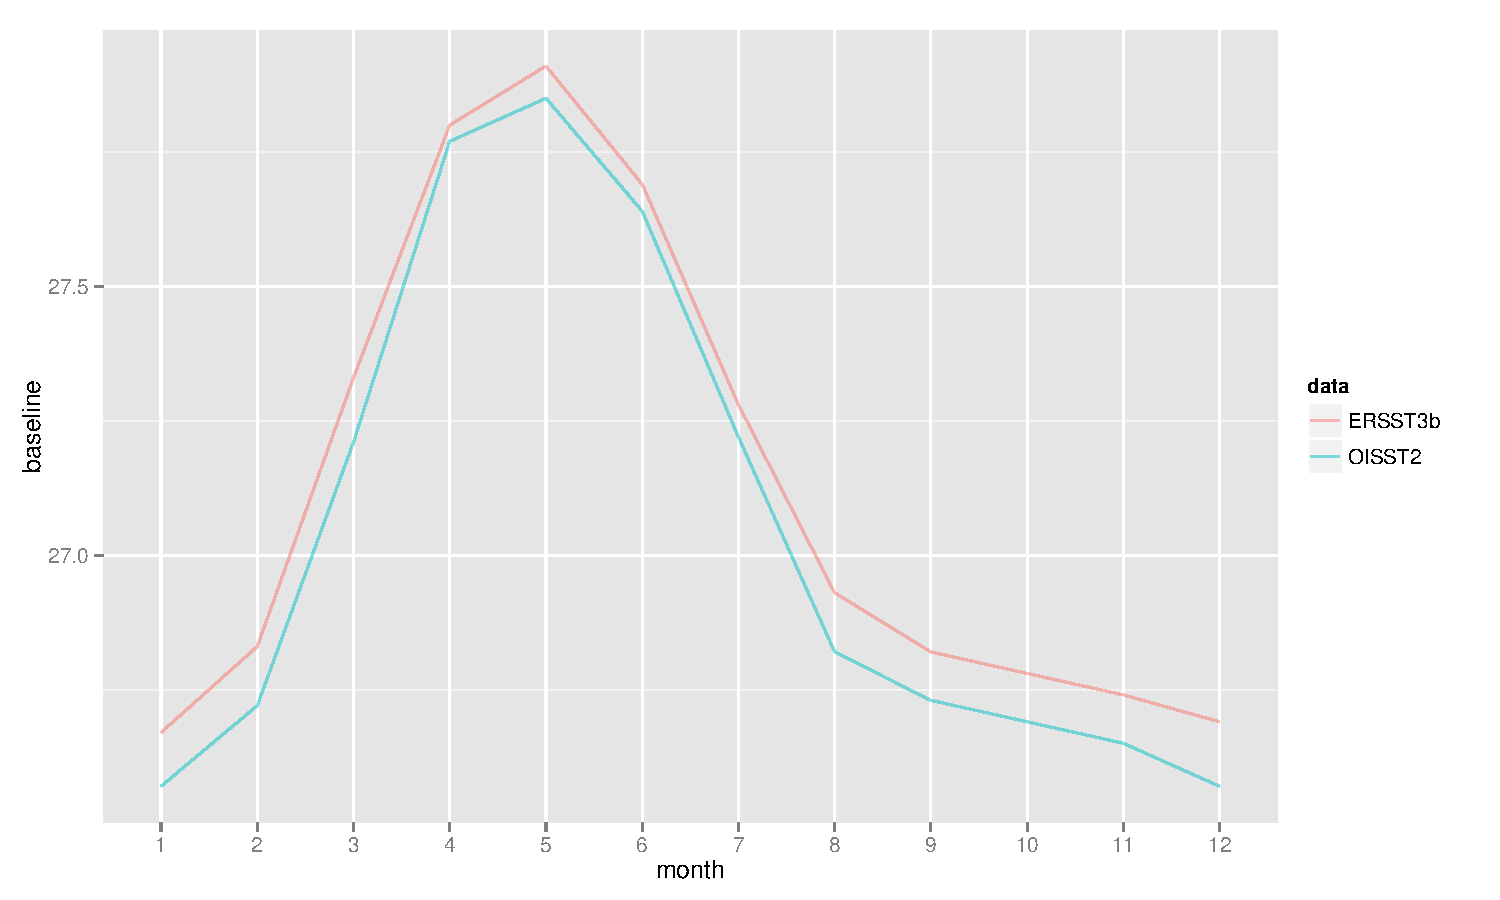
\includegraphics[width=\linewidth]{Pricingfigs/CompareOISSTandERRSTbaselines}
  \caption{Comparing OISST and ERSST monthly baselines}
   \label{fig:baeslinesOIER}
\end{figure*}

Figure \ref{fig:baeslinesOIER} provides the baseline monthly values that NOAA uses to calibrate anomalies in OISST and ERSST. Note OISSTs tendency toward colder SSTs. The cold bias in satellite data is a great concern in the climate literature and is noted in all the index construction papers on ERSST and OISST cited above.

Note also that February/March and June/July are inflection periods, moving both indexes from cold to warm phases (the former months) and back (the latter months). The baseline SST fluctuations over these two windows is dramatic. I suspect that those months will consequently host very active trading, if traded ENSO markets launch. Those are also likely to be the months where climate expertise and proprietary data will provide the largest edge to traders. The possibility of information asymmetries in those months may undermine the volume boost that traded markets might otherwise get from increased volatility. \index{sea-surface temperature!phases}

\paragraph{Result}
ERSST

\subsubsection{Ni\~no region}
Ni\~no 1.2 is the best predictor of catastrophic flooding in Peru and Ecuador, El Ni\~no's flagship impact. However, NMS generally mark ENSO anomalies using the Ni\~no 3.4 region\footnote{Ni\~no 3.4, straddles two separate regions, Ni\~no 3 and Ni\~no 4.} (roughly, from $5\degreesym$N to $5\degreesym$S and from $120\degreesym$ to $170\degreesym$W), which stretches across the central Pacific\cite{khalil2007Nino} \cite{barnston1997documentation}. Both regions, Ni\~no 1.2 and the Ni\~no 3.4, have a very high correlation during extreme anomalies. But Ni\~no 3.4 is generally considered a better proxy for the worldwide teleconnections associated with ENSO. In particular,  it does a better job capturing ENSO anomalies with different geographic signatures. During the 1972/1973 El Ni\~no, for example, most of the sea-surface temperature warming occurred in the central Pacific, closer to Ni\~no 3.4. El Ni\~no events focused on the Central Pacific are also called \emph{Modoki} Ni\~nos and can have large global impacts\cite{ashok2007Nino}.

\paragraph{Result}
use Ni\~no 3.4…

\subsubsection{Anomalies vs. absolute SST measurements}
NOAA releases each of its datasets as departures from monthly averages (anomalies) and absolute degrees Celsius. Its not immediately clear which format is better for financial contracts.

Presenting contracts in terms of anomalies facilitates interpretation of actual El Ni\~no/La Ni\~na events, since most major meteorological organizations define those events in terms of persistent monthly anomalies. Indeed, many forecasts of SSTs (like those from the ABM and IRI) are only provided in terms of anomalies. 

The primary disadvantage of anomalies is that they have been, and will continue to be, subject to revision as underlying SSTs drift over time. 

[THERE IS] a possible [BUT WEAK] link between climate change and higher Pacific SSTs. 

To the extent that such trends continue, the index may revise its baseline and the interpretation of anomalies may become less clear. The ONI index, which NOAA uses to define El Ni\~no/La Ni\~na already uses a rolling window for its monthly base periods.

The weather traders I interviewed [give context] suggested that the temperature derivatives are currently subject to annual revision. The practice has not been a problem for traders. Nevertheless, there may be advantages to using absolute SSTs. Absolute measurements will directly incorporate any underlying shifts in the index, allowing, for example, traders to simply express theories about the long-term trends in the index. Those theories and, by proxy, the market's judgment of long-term climate change might be obscured in an anomaly-based contract.

\subsection{Developing a prototypical contract}
According to Dr. Andrew Watkins of the Australian Bureau of Meteorology (ABM), October is the single most decisive month for El Ni\~no/La Ni\~na worldwide. It is consequently the month I use for most of the examples in this chapter.


I am most concerned with extreme El Ni\~no/La Ni\~na, so I've chosen to structure the payout functions for my example options around events between one and three standard deviations away from the monthly mean. More specifically, payments on the options begin at one standard deviation\footnote{This is also called the trigger or attachment point.} above or below the monthly average (for El Ni\~no coverage/calls and La Ni\~na coverage/puts respectively) and payments reach one hundred percent of the notional value (or sum insured) at three standard deviations above or below the monthly average. Figure \ref{fig:optionParamsByMonth} shows the average monthly value for Ni\~no 3.4 in black. The red and blue bands show the index values for each month that would trigger a payment on calls and puts respectively. \index{risk management contracts!payout function}

\begin{figure*}[!htbp]
  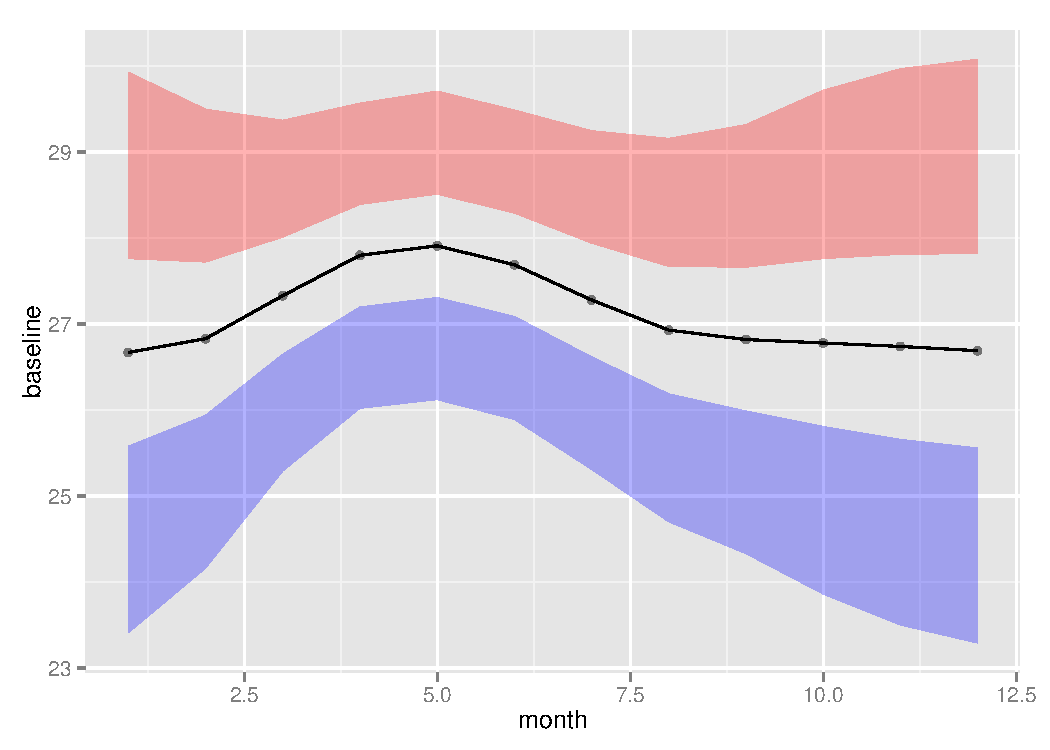
\includegraphics[width=\linewidth]{Pricingfigs/optionParamsByMonth}
  \caption{Index values for El Ni\~no (red) and La Ni\~na (blue) events between one and three standard deviations away from monthly average}
   \label{fig:optionParamsByMonth}
\end{figure*}

Within those ranges, I use linear pricing such that an index value halfway across the red band in figure \ref{fig:optionParamsByMonth} (i.e. halfway between the the trigger and max payout point) would obligate a payout that is half of the sum insured on a call/El Ni\~no contract. The full linear function for October El Ni\~no is shown in figure \ref{fig:payouyt10callex}. 

\begin{figure*}[!htbp]
  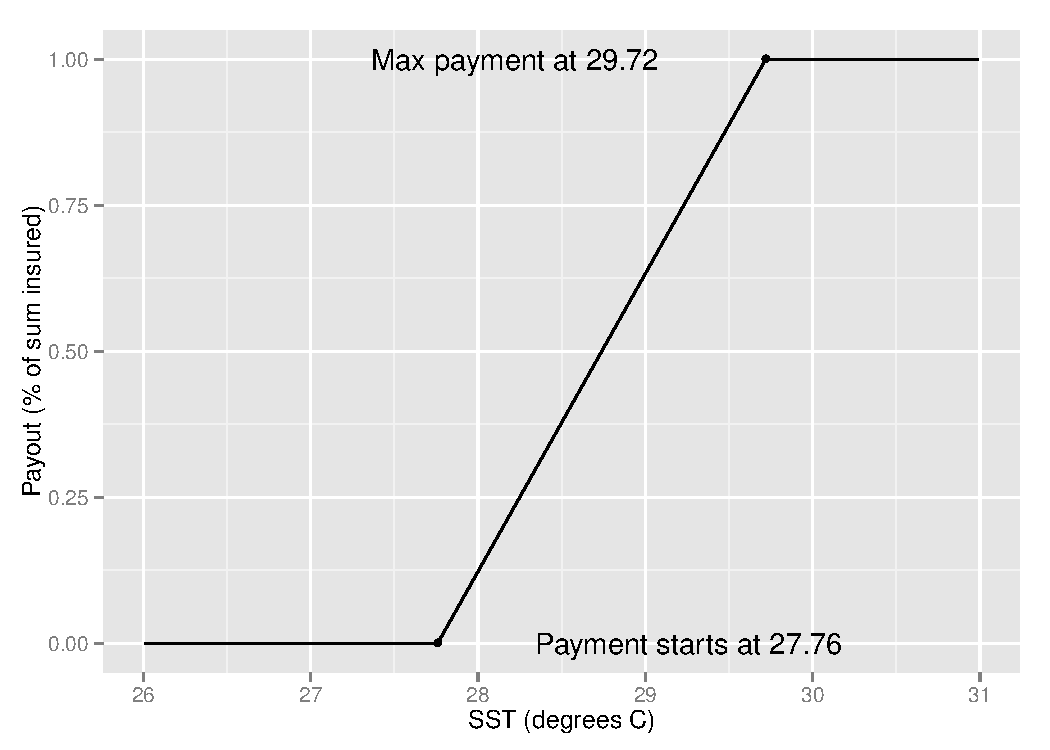
\includegraphics[width=\linewidth]{Pricingfigs/payoutExamplemonth10contractType1}
  \caption{Payout function for call option on October SST for Ni\~no 3.4 ERSST.3b covering index values between one and three standard deviations above the baseline}
   \label{fig:payouyt10callex}
\end{figure*}

As an example, suppose that I bought USD $100$ of coverage for USD $10$ against October El Ni\~no. If actual October SST was halfway across the red band, or $28.74^{\circ}\mathrm{C}$, I would receive USD $50$.

In practice, GlobalAgRisk found that hedgers (and speculators) prefer a payout function that offers a minimum payout in the event that the index reaches just above the trigger. For example, an index value that just barely crosses into the red in \ref{fig:optionParamsByMonth} might trigger a payout of $5$ percent on an El Ni\~no/call contract, rather than the tiny payout suggested the kind of linear function in figure \ref{fig:payouyt10callex}.

Some potential clients also expressed interest in a more customized payout function consisting of steps usually shaped around historical events e.g. a 25 percent payout for the 1972/1973 magnitude event and a 75 percent for a 1997/1998 magnitude event.
\subsubsection{Result}
suggest 1-3 s.d. coverage, put and call

\subsection{Distribution}

In figure \ref{fig:optionPricesWithVariousDistMonth}, I show the prices generated (in USD of premium per USD 100 of nominal coverage) from the random samples from fit distributions. The figure includes burn prices and prices from samples taken from kernel density smoothers fit over each month. 

\begin{figure*}[!htbp]
  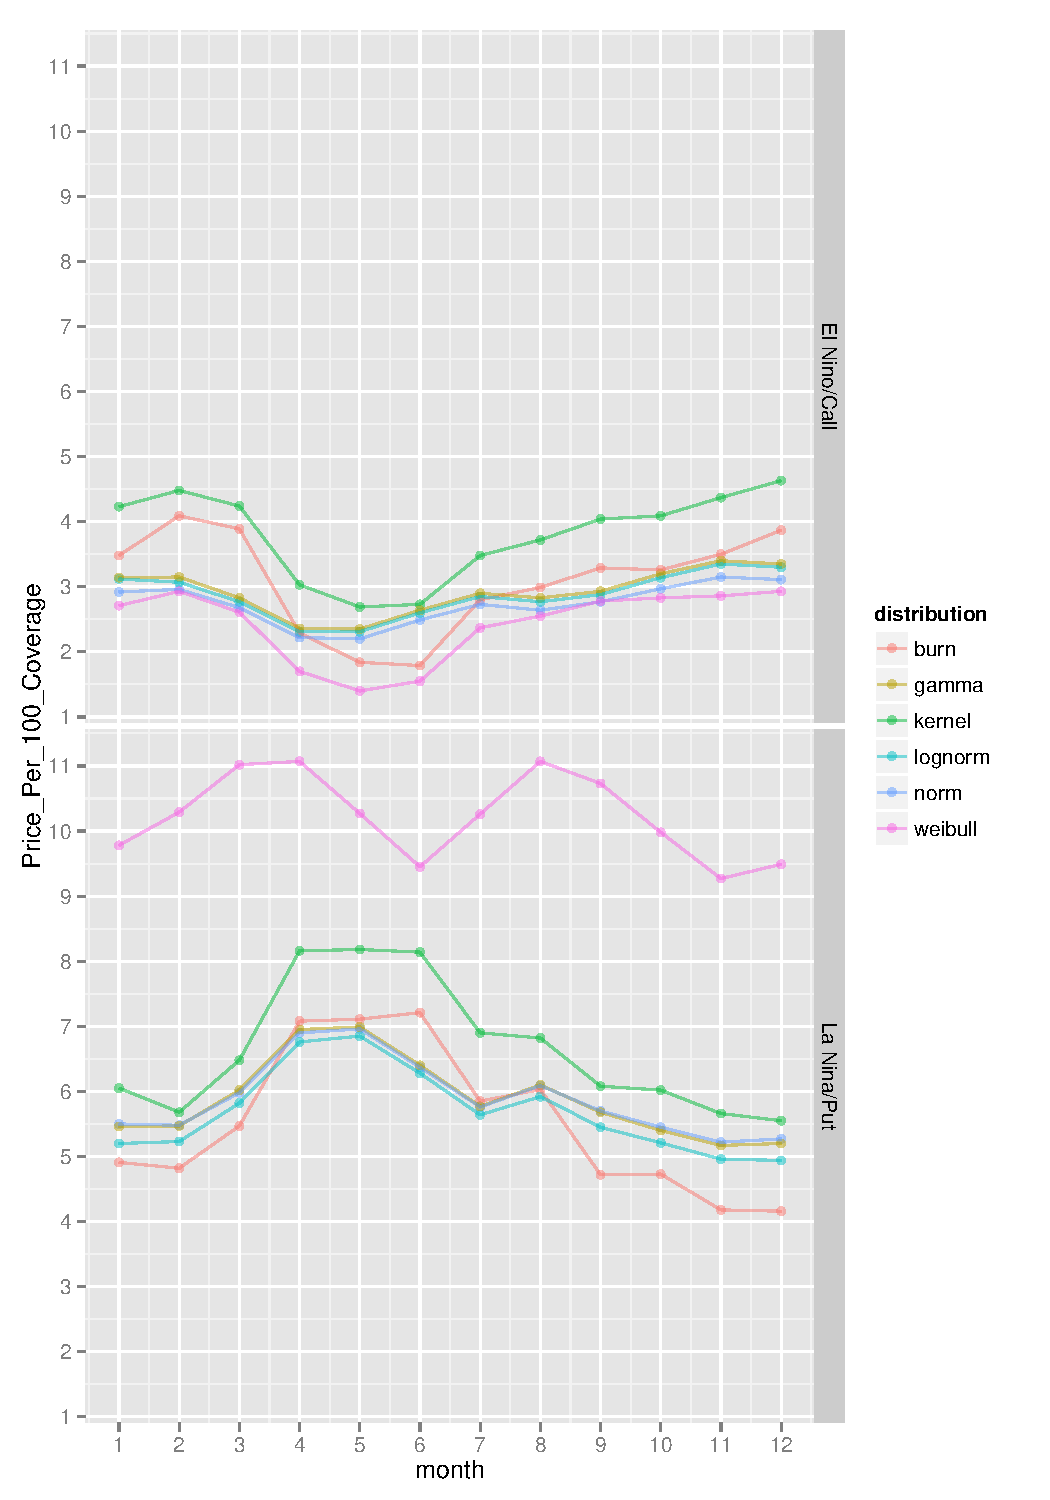
\includegraphics[width=\linewidth]{Pricingfigs/optionPricesWithVariousDistMonth}
  \caption{Expected price for options on Ni\~no 3.4 by month, based on simulations from various distributions}
   \label{fig:optionPricesWithVariousDistMonth}
\end{figure*}

The prices from the various distributions are, with one prominent exception, close together. On the El Ni\~no side, the highest and lowest prices are mostly within 125 basis points of one another in any given month. On the La Ni\~na side, that spread is slightly larger at roughly 150 basis point, but only between April and June.

The Weibull, is the one model challenging this consensus. The prices from the Weibull samples are clearly distinct from the rest of the group - almost doubling the price of La Ni\~na coverage relative to the rest of the group. The Weibull sample suggested the lowest prices for El Ni\~no coverage, albeit by a much smaller margin than for La Ni\~na. That is understandable given the distribution's heavy left tail.

Apart from the Weibull, the samples drawn from the kernel density smoother suggests the second highest prices for both El Ni\~no and La Ni\~na coverage. The burn prices are in the middle of the pack.
\subsubsection{Result}
robust to several distributional assumptions. 
Using normal has advantages

\subsection{Picking a forecast}
Forecasts, IRI’s ensemble, and error around the ensemble forecast
\subsubsection{Result 1}
IRI ensemble good foundation for baseline

\subsection{Pricing ensemble error}

Extreme El Ni\~no/La Ni\~na events emerge over time, with forecasts giving us even more useful hints in the months leading up to a given event. As those hints emerge, we change our beliefs around the likelihood of an event. The price of El Ni\~no/La Ni\~na risk protection should change to reflect those beliefs.

In this section, we present statistical simulations of monthly Ni\~no 3.4 sea surface temperatures conditioned on average forecasts released by Colombia University's International Research Institute for Climate and Society (IRI). We use those simulations to update the prices of risk management contracts as new forecast information becomes available.

Every month since mid-2002, IRI has collected forecasts issued by major centers of climatological research. Figure \ref{fig:forecastExamples} shows IRI the forecasts as of March 2013.

\begin{figure}[!htbp]
  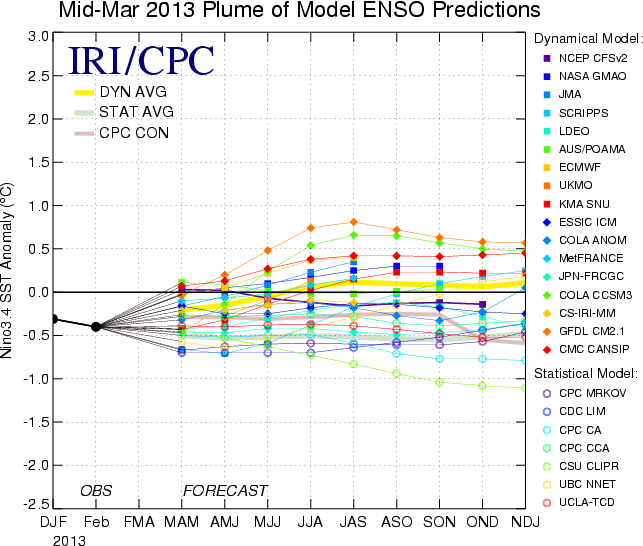
\includegraphics[width=\linewidth]{Pricingfigs/SST_table_march_ex}
  \caption{Example of IRI's collected forecasts - March 2013}
   \label{fig:forecastExamples}
\end{figure}

The work presented here links those forecasts and observed SSTs through a Bayesian regression that uses the long terms climate record as a prior. If the regression indicates that the forecasts have no predictive power, then all the simulated SSTs from the regression will simply reflect monthly historical averages. 

\subsubsection{Modeling the link between forecasts and SSTs}
IRI provides Nino 3.4 SST forecasts are over 3 month rolling windows. However, that format is unlikely to satisfy hedgers. Many would prefer to mix and match the months closest to them. Existing El Ni\~no insurance is based on a Novermber/December average, but some clients in Peru expressed interest in protection against individual months. 

So, for the sake of providing ENSO pricing information of most direct relevance to likely traded markets, we have linked the smoothed IRI forecasts to monthly measured SST. For an example of how we made this link, imagine that it is March and a hedger is interested in predicting October Ni\~no 3.4 SST. IRI's forecasts (given in terms of anomalies) are smoothed using three-month blocks, as in figure \ref{fig:forecastExamples}. In that figure, there are three forecasts that contain information relevant to October SSTs - \emph{ASO}, \emph{SON}, and \emph{OND}. 

There are myriad ways of combining both individual and average forecasts for those three windows in a regression, but for the sake of simplicity in this section we use as the independent variable the average of IRI model averages covering October. 

So, in the above example, I would look at all the model averages made in March for \emph{ASO}, \emph{SON}, and \emph{OND}, taking the average of those three numbers in any given year. I did the same for every month across that months valuable forecasts. That forecast average then conditions the long-term average anomaly for October\footnote{I used anomalies rather than absolute SSTs to match IRI's convention.}. IRI issues forecasts between 2 and 10 months prior to any given target month. For example, October SST forecasts begin in December and end in September. Since I want pricing for every month, from the vantage-point of every preceding month with IRI forecasts, I need to run a total of $108$ separate regressions. 

\begin{equation}
\begin{array}{lcl}
\mbox{Monthly Ni\~no 3.4 ERSST.3b anomalies}_{month,year} & \sim & \mathcal{N}( \hat{y}_{month,forecast month,year}, \sigma_{y_{month,forecast month}}^2 )\\
\hat{y}_{month,forecast month,year} & = & a_{month,forecast month} \\
&& + b_{month,forecast month}*\\
&& \mbox{average of IRI average forecasts}_{month,forecast month}\\
\end{array}
\label{eqn:conditionalEstEqn}
\end{equation}

Those regressions, specified in equation \ref{eqn:conditionalEstEqn}, are a simplified version of a procedure that climate scientists and statisticians have recently used to merge ENSO forecasts\cite{luo2007bayesian}\cite{coelho2004forecast}. Note first that I do not know the predictive power of IRI average forecasts. The parameter $\sigma_{y_{month,forecast month}}^2$ accounts for that forecasting uncertainty. It will be large where IRI average forecasts have shown low historical predictive power. Note also that this Bayesian regression will not be biased by non-stationarity. The underlying parameters are not assumed to be stationary, since they are realizations of an unknown distribution.

The prior probabilities I placed on model parameters are shown in equation set \ref{eqn:priorsconditionalEstEqn}. There are weakly informative priors on $b$ and $\sigma_{y}$, allowing them to move easily across a wide range of possible values in response to the data. $a$ by contrast has a strongly informative prior based on historical data. This means that if $b$, the parameter indicating the predictive power of IRI's average forecasts, is at or near zero, then the resulting simulations from the posterior distribution will simply reflect long term trends in monthly SSTs.

\begin{equation}
\begin{array}{lcl}
a_{month,forecast month}  & \sim & \mathcal{N}(\mbox{mean anomalies}_{month}, \mbox{st dev anomalies}_{month}) \\
b_{month,forecast month}  & \sim & \mathcal{N}(0, 100) \\
\sigma_{y_{month,forecast month}}^2 & \sim  &\mbox{Inv gamma}(0.001, 0.001) \\
\end{array}
\label{eqn:priorsconditionalEstEqn}
\end{equation}

\subsubsection{Dynamic pricing based on model results}
The table below contains regression results for October SSTs, predicted between the preceding December and August. The regressions were all estimated using parallel Markov Chain Monte Carlo (MCMC) chains, each with 100,000 iterations, 50,000 of which were discarded as a warm-up\cite{stan2013}. 

[CHANGE]
The $\hat{R}$ on all parameters below and in part Pricing Appendix were 1, indicating convergence on the simulation.

\begin{table*}[ht]
\centering
\footnotesize
\begin{tabular}{rrrrrrrrrr}
\hline
\multicolumn{10}{c}{August forecast average covering October Ni\~no 3.4 SST anomalies}\\

  \hline
 & mean & sd & $2.5^{\mbox{th}}$ q & $25^{\mbox{th}}$ q & $50^{\mbox{th}}$ q & $75^{\mbox{th}}$ q & $97.5^{\mbox{th}}$ q & n\_eff & Rhat \\ 
  \hline
$\alpha$ & -0.10 & 0.10 & -0.40 & -0.20 & -0.10 & -0.10 & 0.10 & 91045 &   1 \\ 
  $\beta$ & 1.10 & 0.20 & 0.80 & 1.00 & 1.10 & 1.20 & 1.50 & 88920 &   1 \\ 
  $\sigma^{2}_{y}$ & 0.10 & 0.10 & 0.10 & 0.10 & 0.10 & 0.20 & 0.40 & 56829 &   1 \\ 
   \hline
\hline
\multicolumn{10}{c}{July forecast average covering October Ni\~no 3.4 SST anomalies}\\
  \hline
$\alpha$ & -0.10 & 0.20 & -0.50 & -0.20 & -0.10 & 0.00 & 0.20 & 92218 &   1 \\ 
  $\beta$ & 1.20 & 0.30 & 0.60 & 1.00 & 1.20 & 1.30 & 1.70 & 93712 &   1 \\ 
  $\sigma^{2}_{y}$ & 0.30 & 0.20 & 0.10 & 0.20 & 0.30 & 0.40 & 0.90 & 54297 &   1 \\ 
   \hline
\hline
\multicolumn{10}{c}{June forecast average covering October Ni\~no 3.4 SST anomalies}\\
  \hline
$\alpha$ & -0.10 & 0.20 & -0.40 & -0.20 & -0.10 & 0.00 & 0.30 & 95908 &   1 \\ 
  $\beta$ & 1.40 & 0.30 & 0.70 & 1.20 & 1.40 & 1.60 & 2.10 & 91107 &   1 \\ 
  $\sigma^{2}_{y}$ & 0.30 & 0.20 & 0.10 & 0.20 & 0.30 & 0.40 & 0.90 & 55596 &   1 \\ 
   \hline
\hline
\multicolumn{10}{c}{May forecast average covering October Ni\~no 3.4 SST anomalies}\\
  \hline
$\alpha$ & -0.10 & 0.20 & -0.50 & -0.20 & -0.10 & 0.10 & 0.40 & 92919 &   1 \\ 
  $\beta$ & 1.50 & 0.60 & 0.40 & 1.20 & 1.50 & 1.90 & 2.60 & 90255 &   1 \\ 
  $\sigma^{2}_{y}$ & 0.50 & 0.30 & 0.20 & 0.30 & 0.50 & 0.60 & 1.40 & 59205 &   1 \\ 
   \hline
\hline
\multicolumn{10}{c}{April forecast average covering October Ni\~no 3.4 SST anomalies}\\
  \hline
$\alpha$ & -0.10 & 0.20 & -0.50 & -0.30 & -0.10 & 0.00 & 0.30 & 88326 &   1 \\ 
  $\beta$ & 1.90 & 0.60 & 0.70 & 1.50 & 1.90 & 2.30 & 3.00 & 83902 &   1 \\ 
  $\sigma^{2}_{y}$ & 0.40 & 0.30 & 0.20 & 0.30 & 0.40 & 0.50 & 1.10 & 57674 &   1 \\ 
   \hline
\hline
\multicolumn{10}{c}{March forecast average covering October Ni\~no 3.4 SST anomalies}\\
  \hline
$\alpha$ & 0.00 & 0.20 & -0.50 & -0.10 & 0.00 & 0.20 & 0.50 & 101040 &   1 \\ 
  $\beta$ & 1.80 & 0.90 & 0.00 & 1.20 & 1.80 & 2.30 & 3.50 & 96782 &   1 \\ 
  $\sigma^{2}_{y}$ & 0.70 & 0.50 & 0.30 & 0.50 & 0.60 & 0.90 & 1.90 & 59539 &   1 \\ 
   \hline
\hline
\multicolumn{10}{c}{February forecast average covering October Ni\~no 3.4 SST anomalies}\\
  \hline
$\alpha$ & -0.10 & 0.30 & -0.70 & -0.30 & -0.10 & 0.10 & 0.60 & 98192 &   1 \\ 
  $\beta$ & 0.80 & 1.30 & -1.80 & 0.00 & 0.80 & 1.60 & 3.40 & 88684 &   1 \\ 
  $\sigma^{2}_{y}$ & 1.10 & 0.80 & 0.40 & 0.60 & 0.90 & 1.30 & 3.20 & 54912 &   1 \\ 
   \hline
\hline
\multicolumn{10}{c}{January forecast average covering October Ni\~no 3.4 SST anomalies}\\
  \hline
$\alpha$ & 0.00 & 0.30 & -0.60 & -0.20 & 0.00 & 0.20 & 0.60 & 99518 &   1 \\ 
  $\beta$ & 1.00 & 1.60 & -2.30 & 0.00 & 1.00 & 2.00 & 4.20 & 92225 &   1 \\ 
  $\sigma^{2}_{y}$ & 1.00 & 0.70 & 0.40 & 0.60 & 0.80 & 1.20 & 2.80 & 55715 &   1 \\ 
   \hline
\hline
\multicolumn{10}{c}{December forecast average covering October Ni\~no 3.4 SST anomalies}\\
  \hline
$\alpha$ & 0.00 & 0.30 & -0.60 & -0.20 & 0.00 & 0.30 & 0.70 & 80946 &   1 \\ 
  $\beta$ & -0.30 & 1.90 & -4.00 & -1.40 & -0.30 & 0.90 & 3.50 & 76663 &   1 \\ 
  $\sigma^{2}_{y}$ & 1.10 & 0.70 & 0.40 & 0.60 & 0.90 & 1.30 & 2.90 & 56323 &   1 \\ 
   \hline
\end{tabular}
\caption[Bayesian regression linking October Ni\~no 3.4 SST anomalies to average of relevant IRI ensemble forecasts]{Bayesian regression linking October Ni\~no 3.4 SST anomalies to average of relevant IRI ensemble forecasts} 
\end{table*}


Looking at the 2.5th and 97.5th percentile of the distributions for $b$, its clear that the forecasts become more valuable predictors as the year goes on. Going from December to August, the 95 percent probability interval for the forecast parameter, $b$ steadily tightens to a range including 1. This suggest that the correlation between forecasts and eventual SSTs increases throughout the predictive window. As the explanatory value of $b$ increases, $a$ decreases. Just as climate scientists suggested, $a$'s 95 percent probability tightening around 0 after March.

Using the posterior draws of parameter values from these 108 regressions, I simulated SSTs predicted by each possible forecast value between -2 and 2 (forecasts are rounded to one decimal). For example, I took 50,000 posterior draws of $a$, $b$, and $\sigma_{y}^2$ from the regression corresponding to October SSTs predicted by April forecasts. I used each of those 50,000 vectors of three parameters to randomly generate one October SSTs, based on an average April forecast of mild El Ni\~no conditions in the coming October (a forecast value of 0.5.) That left me with 50,000 October SST conditioned on a forecast of 0.5 made in April. I repeated that procedure to produce conditional distributions for SSTs for each month of the year, predicted by a wide range of forecast values, from all possible forecast months. The resulting stochastic catalog allowed me to price El Ni\~no/La Ni\~na risk for any month given any IRI average forecast. 

The empirical distribution functions of those posterior simulations, converted back into absolute SSTs, are shown in figures \ref{fig:conditionalCDFs04to06}, \ref{fig:conditionalCDFs07to09}, \ref{fig:conditionalCDFs10to12}, and \ref{fig:conditionalCDFs01to03}. 

For the sake of clarity, simplified illustrative examples of those figures are are presented in \ref{fig:conditionalCDFsIllustrativeExamplesTradConfigFull} and \ref{fig:conditionalCDFsIllustrativeExamplesTradConfigSimple}.

\begin{figure*}[!htbp]
  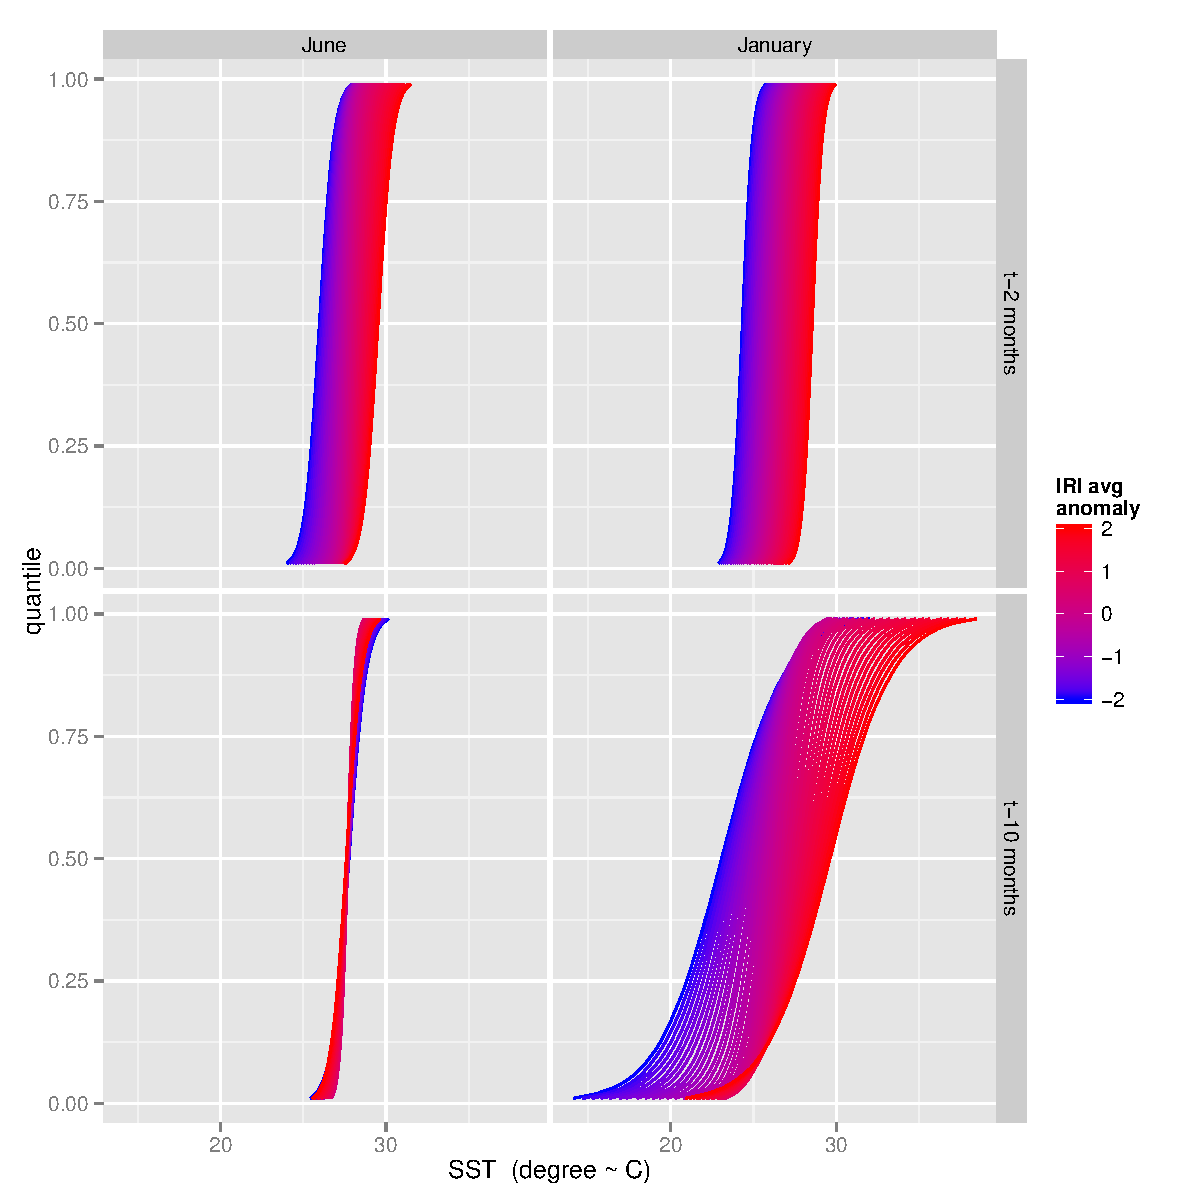
\includegraphics[width=\linewidth]{Pricingfigs/conditionalCDFsIllustrativeExamplesTradConfigFull}
  \caption{Empirical cumulative distribution functions for June and January Ni\~no 3.4 SST conditioned on average IRI ensemble forecasts available for various months. Only the ECDFs for the nearest and furthest month predictions provided by IRI are shown. ECDFs are of draws from the posterior predictive distribution of the model specified in equation \ref{eqn:conditionalEstEqn}.}
   \label{fig:conditionalCDFsIllustrativeExamplesTradConfigFull}
\end{figure*}

\begin{figure*}[!htbp]
  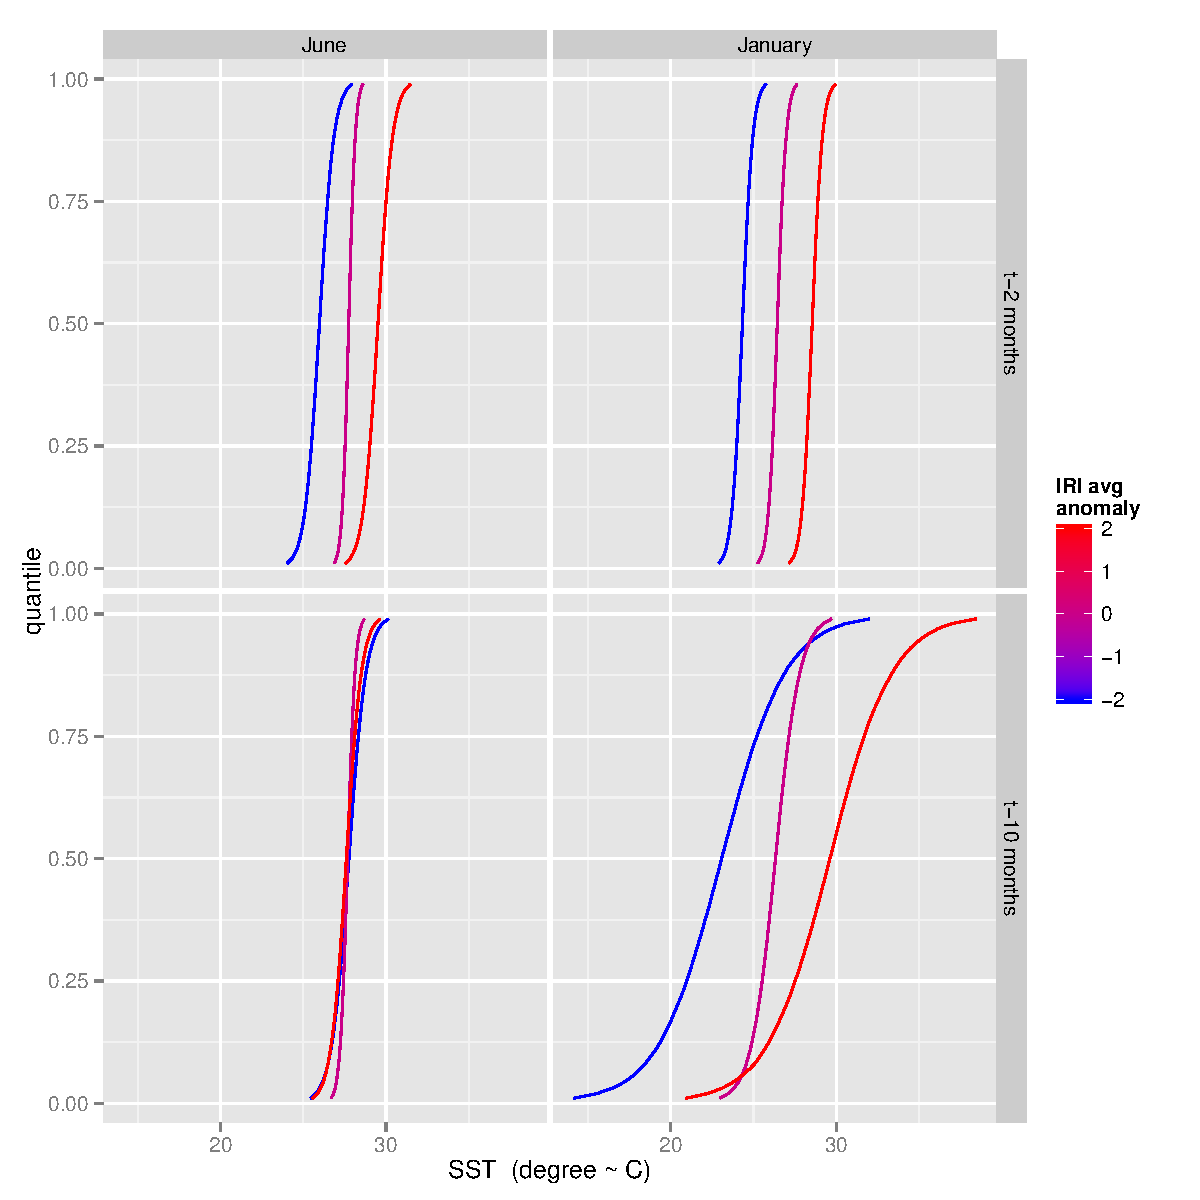
\includegraphics[width=\linewidth]{Pricingfigs/conditionalCDFsIllustrativeExamplesTradConfigSimple}
  \caption{Empirical cumulative distribution functions for June and January Ni\~no 3.4 SST conditioned on average IRI ensemble forecasts available for various months. Only the ECDFs for the nearest and furthest month predictions provided by IRI and only predictions of large El Ni\~no (+2), La Ni\~na (-2), or neutral conditions (0) are shown. ECDFs are of draws from the posterior predictive distribution of the model specified in equation \ref{eqn:conditionalEstEqn}.}
   \label{fig:conditionalCDFsIllustrativeExamplesTradConfigSimple}
\end{figure*}

In those figures, deeper blue lines indicate colder forecast averages from IRI and deeper red lines indicate warmer forecasts.
 
 % fig:conditionalCDFsJantoJune
 % fig:conditionalCDFsJultoDec

% \ref{fig:conditionalCDFsJantoJune} and \ref{fig:conditionalCDFsJultoDec}

 % \ref{fig:conditionalCDFs04to06}, \ref{fig:conditionalCDFs07to09}, \ref{fig:conditionalCDFs10to12}, and  \ref{fig:conditionalCDFs01to03}
\begin{figure*}[!htbp]
  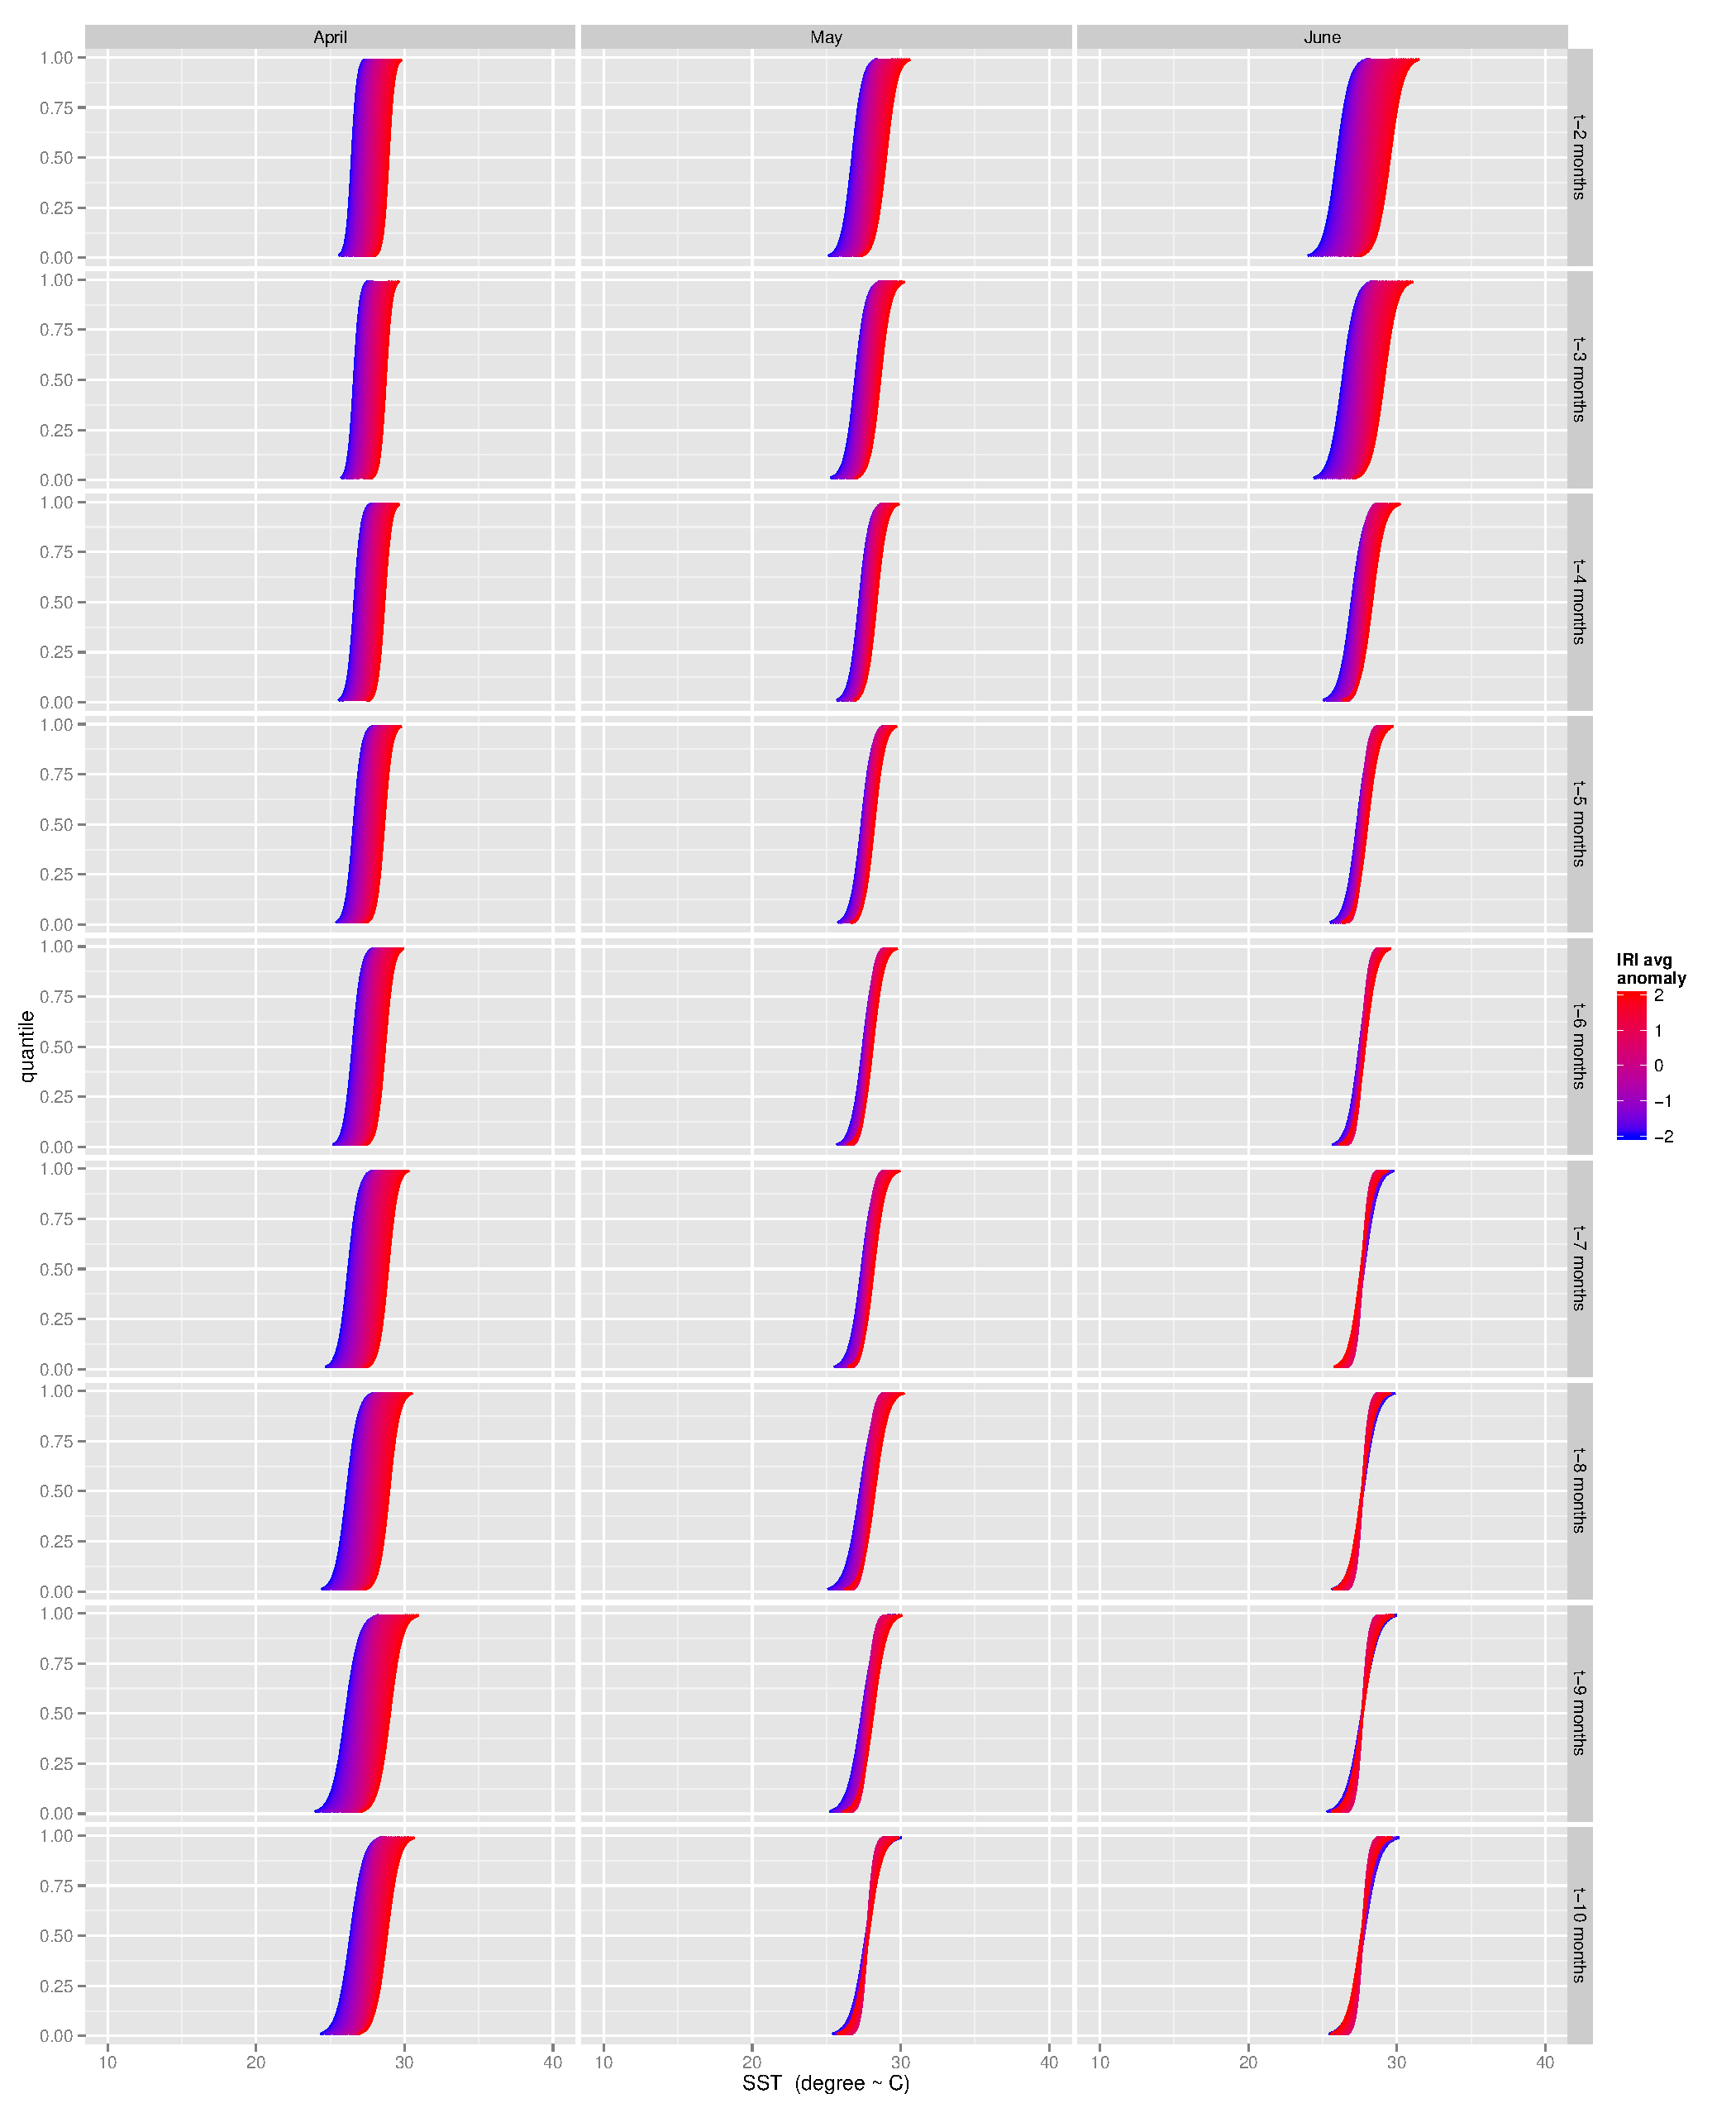
\includegraphics[width=\linewidth]{Pricingfigs/conditionalCDFs04to06TraditionalCDFconfig}
  \caption{Empirical cumulative distribution functions for April through June Ni\~no 3.4 SST conditioned on average IRI ensemble forecasts available for various months. ECDFs are of draws from the posterior predictive distribution of the model specified in equation \ref{eqn:conditionalEstEqn}.}
   \label{fig:conditionalCDFs04to06}
\end{figure*}

\begin{figure*}[!htbp]
  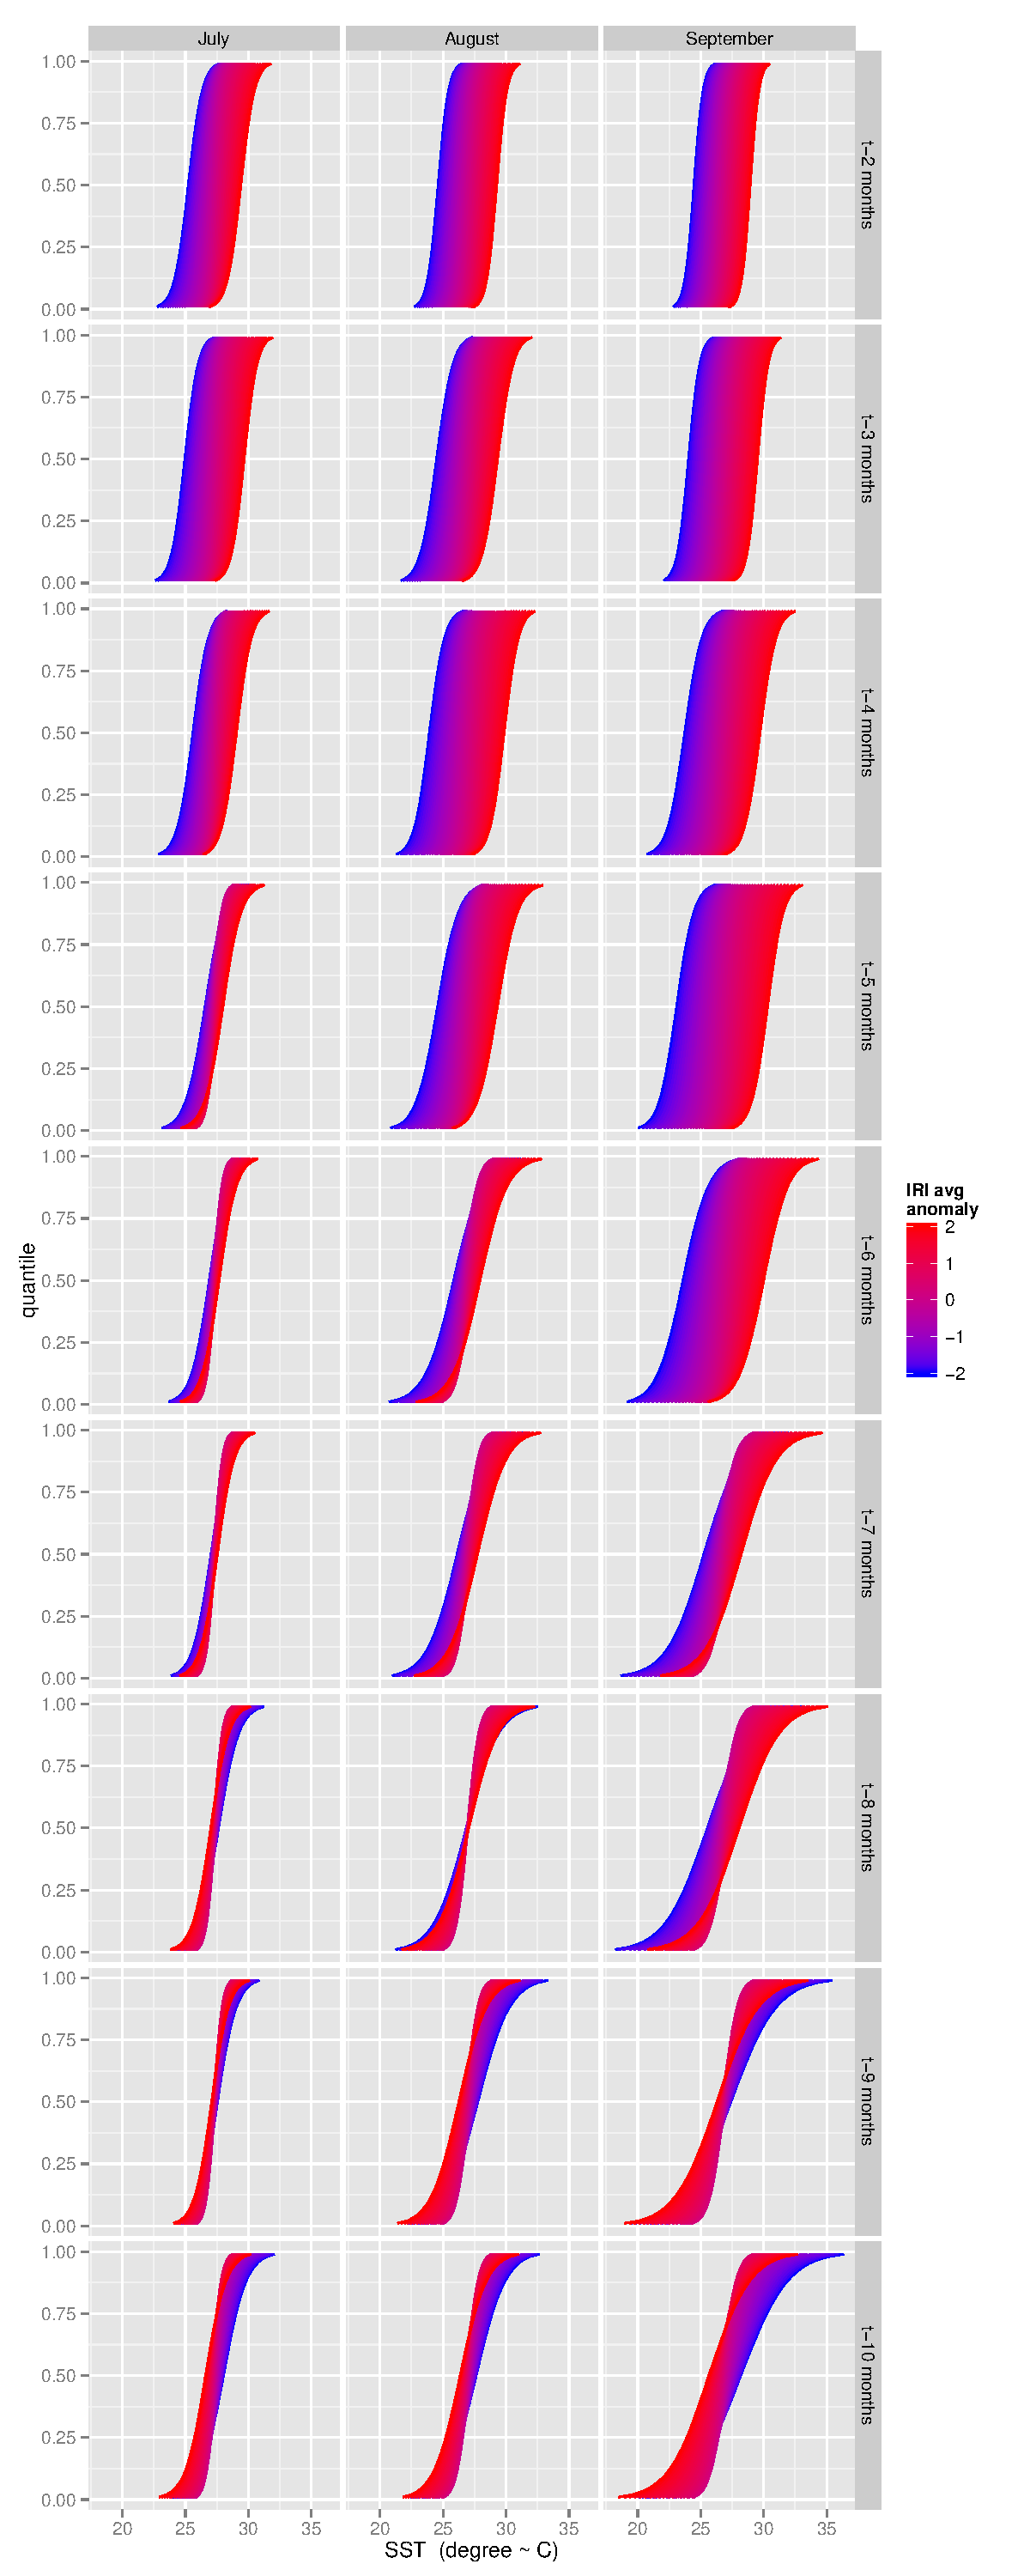
\includegraphics[width=\linewidth]{Pricingfigs/conditionalCDFs07to09TraditionalCDFconfig}
  \caption{Empirical cumulative distribution functions for July through September Ni\~no 3.4 SST conditioned on average IRI ensemble forecasts available for various months. ECDFs are of draws from the posterior predictive distribution of the model specified in equation \ref{eqn:conditionalEstEqn}.}
   \label{fig:conditionalCDFs07to09}
\end{figure*}

\begin{figure*}[!htbp]
  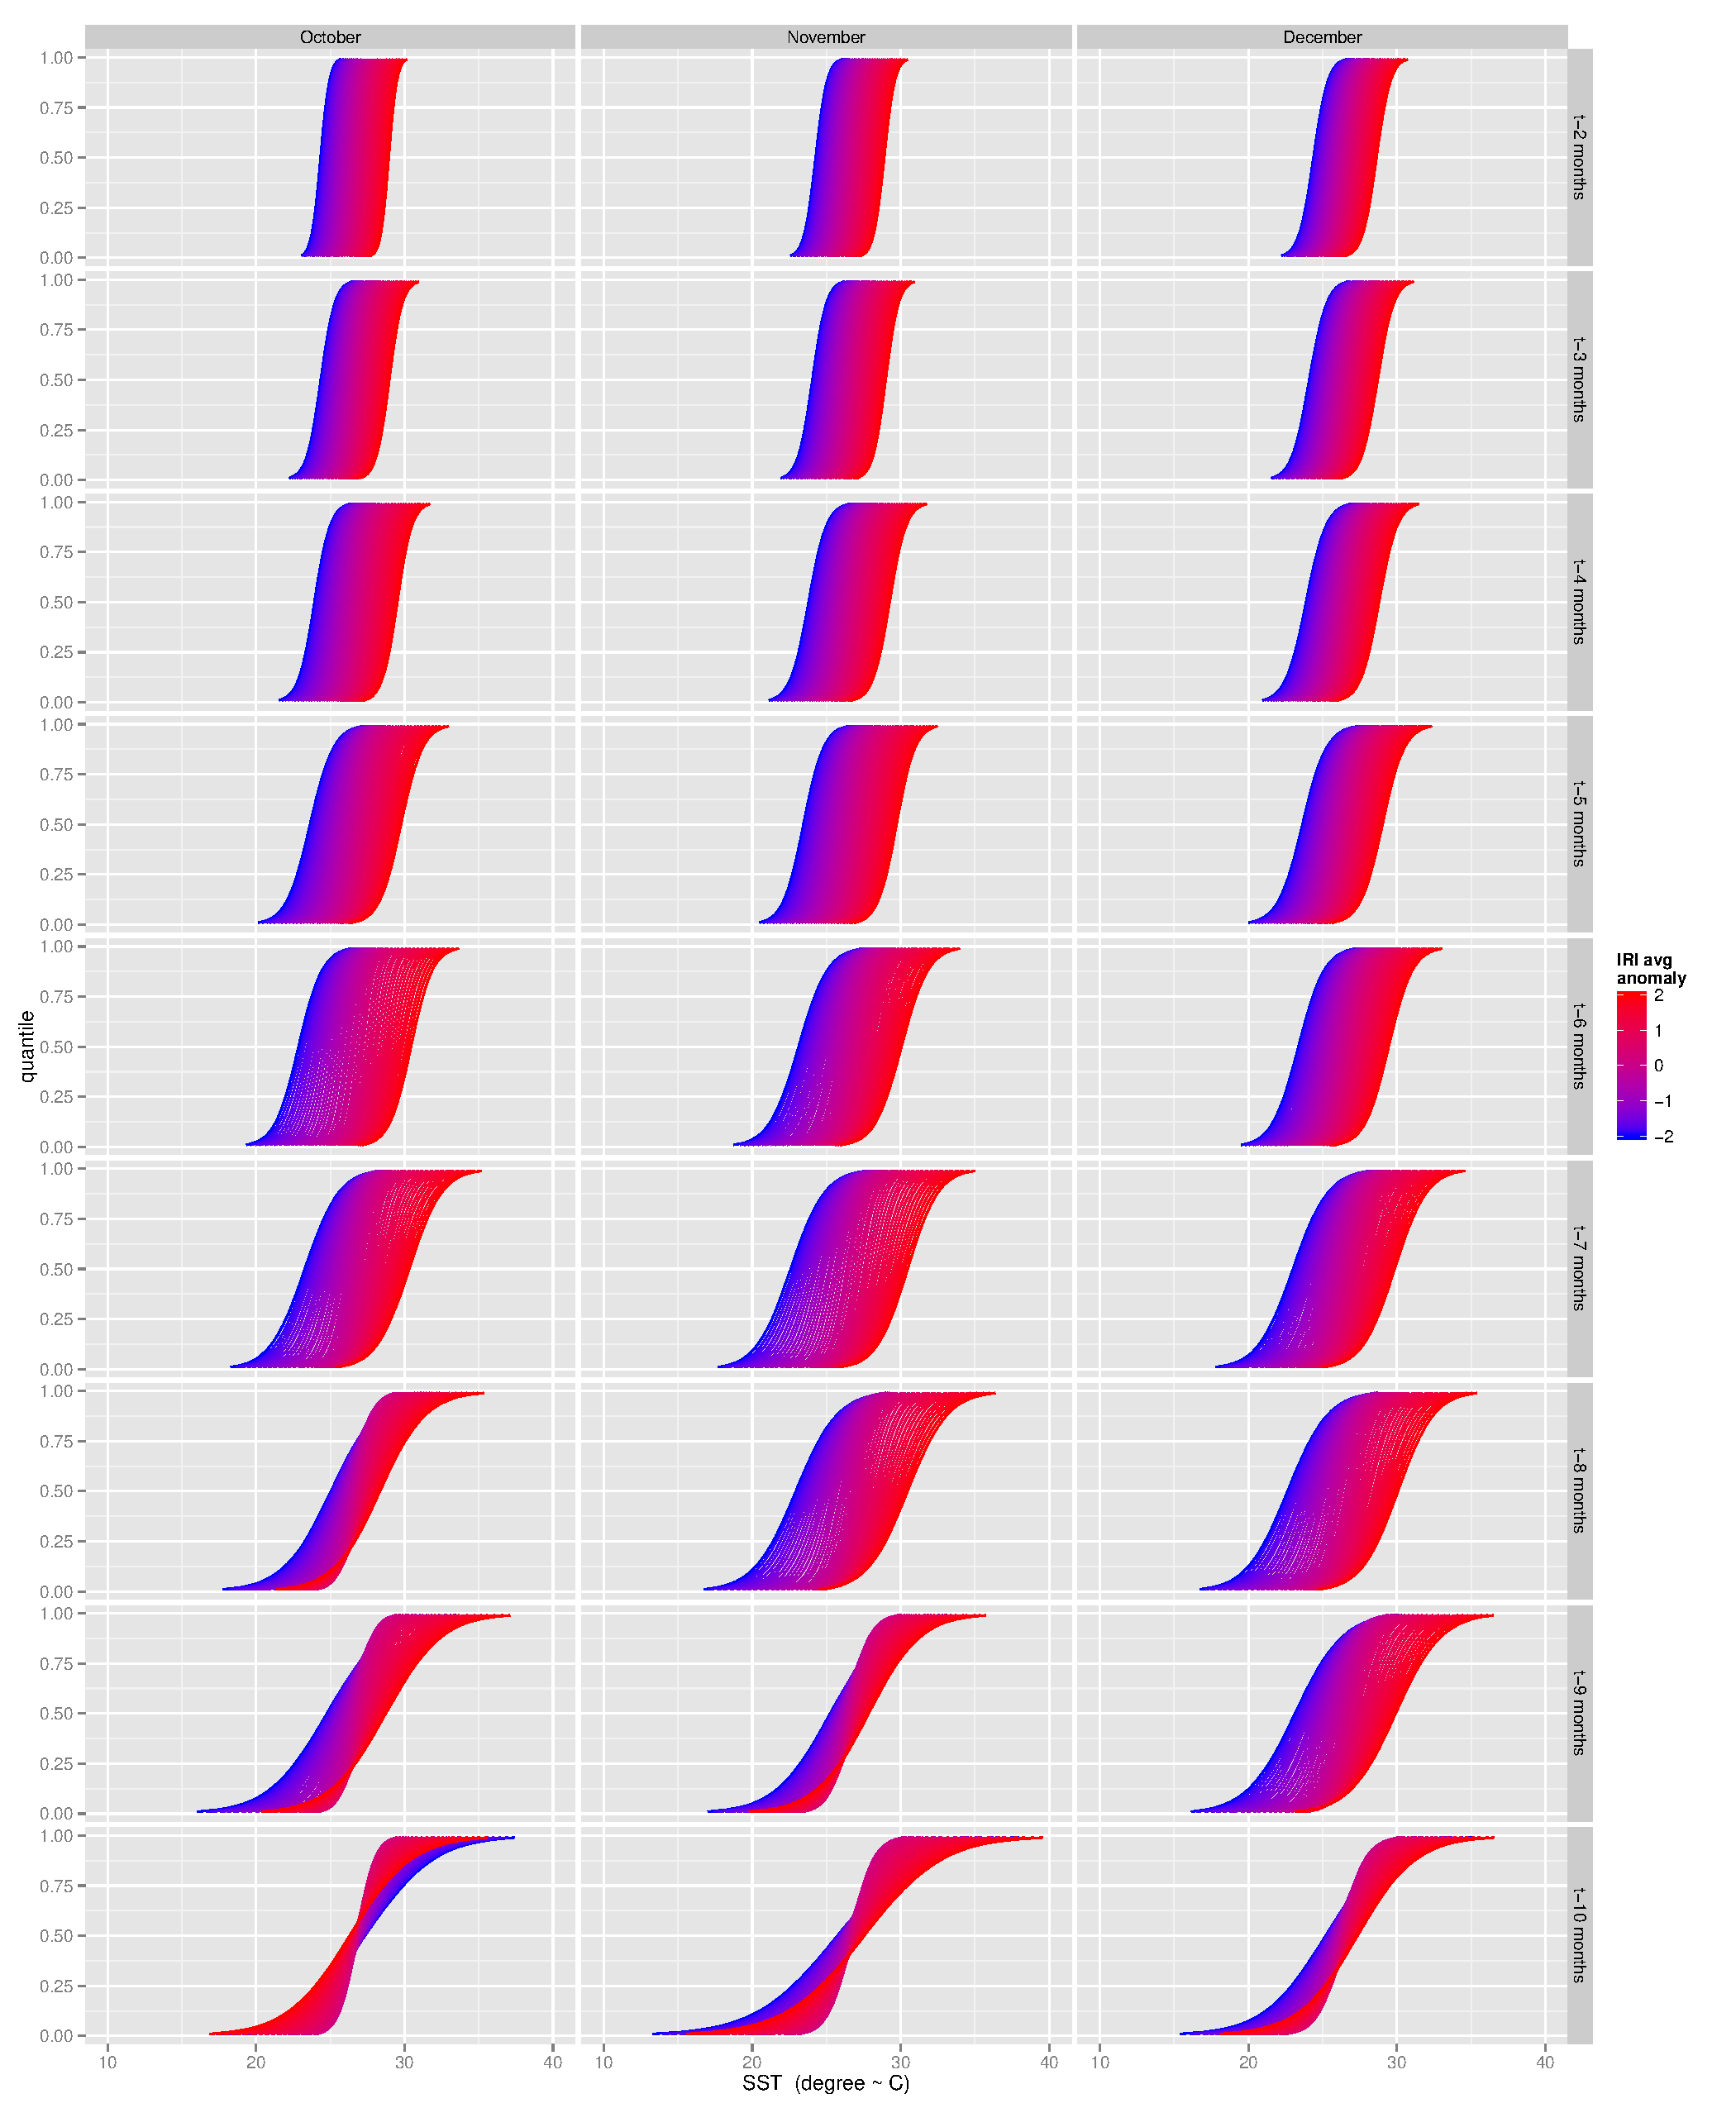
\includegraphics[width=\linewidth]{Pricingfigs/conditionalCDFs10to12TraditionalCDFconfig}
  \caption{Empirical cumulative distribution functions for October through December Ni\~no 3.4 SST conditioned on average IRI ensemble forecasts available for various months. ECDFs are of draws from the posterior predictive distribution of the model specified in equation \ref{eqn:conditionalEstEqn}.}
   \label{fig:conditionalCDFs10to12}
\end{figure*}

\begin{figure*}[!htbp]
  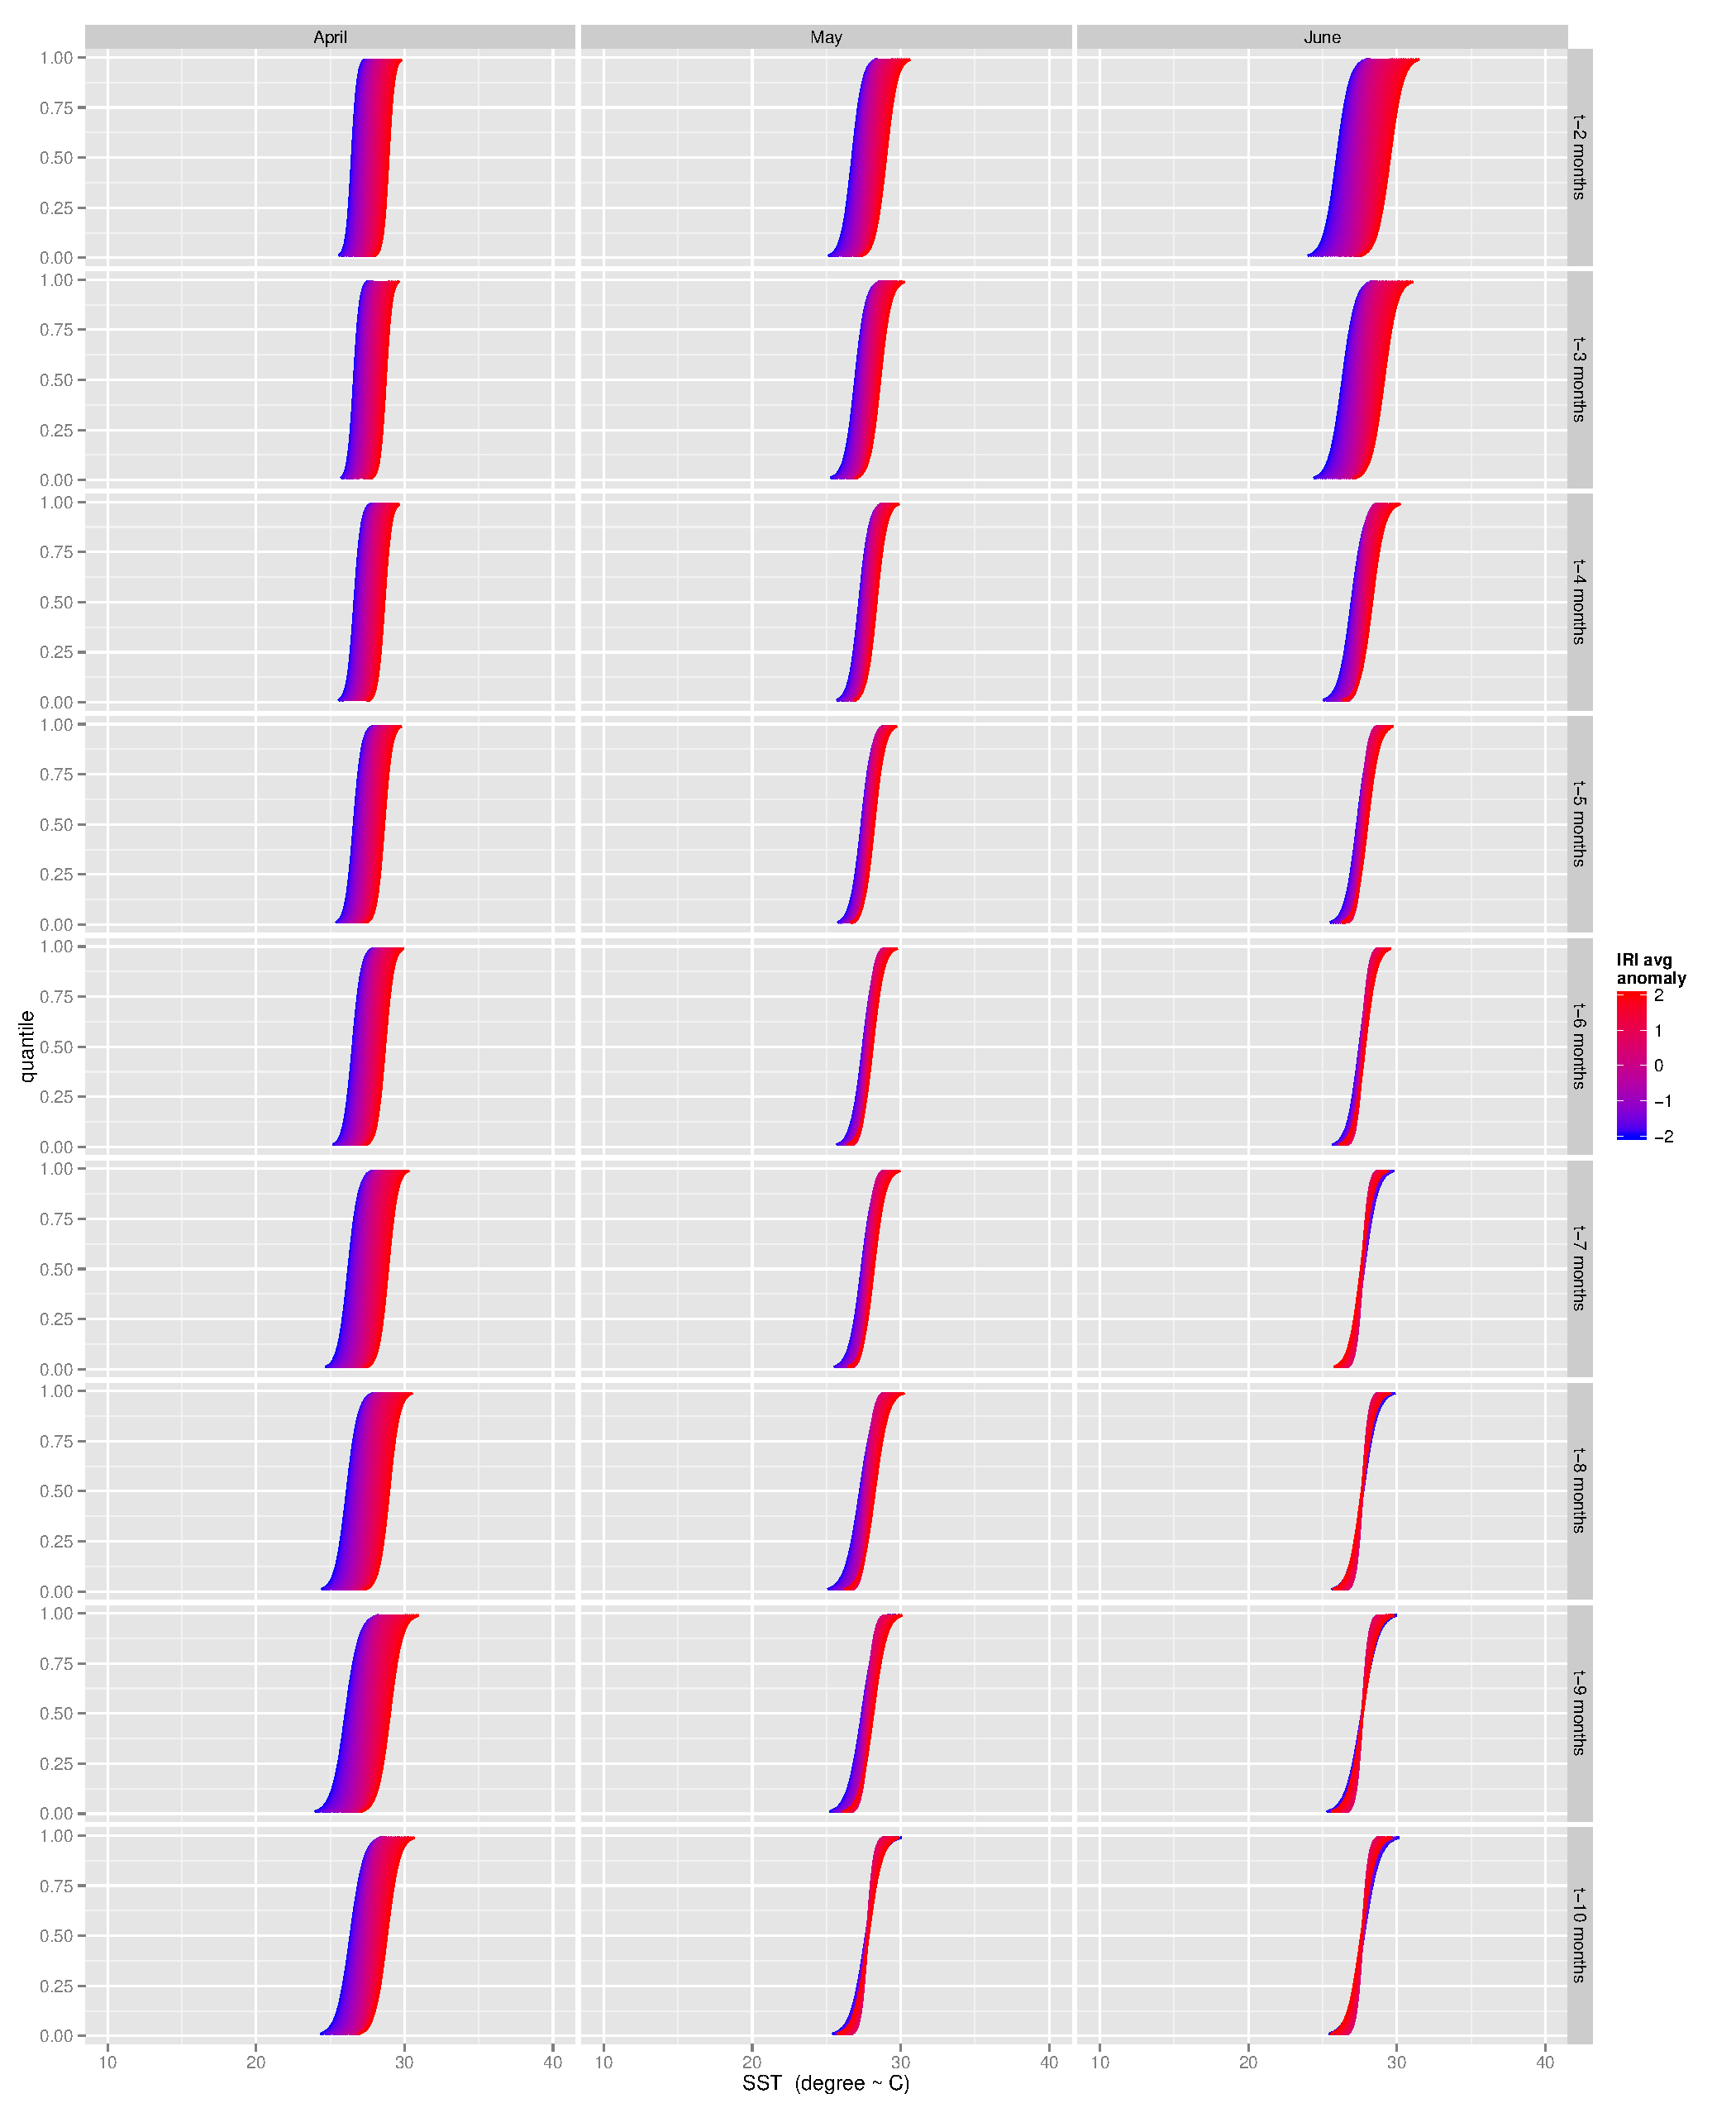
\includegraphics[width=\linewidth]{Pricingfigs/conditionalCDFs04to06TraditionalCDFconfig}
  \caption{Empirical cumulative distribution functions for January through March Ni\~no 3.4 SST conditioned on average IRI ensemble forecasts available for various months. ECDFs are of draws from the posterior predictive distribution of the model specified in equation \ref{eqn:conditionalEstEqn}.}
   \label{fig:conditionalCDFs01to03}
\end{figure*}

Notice how the blue and red lines are tightly bound ten months prior to any given target month (down the rightmost column) in figures \ref{fig:conditionalCDFs04to06}, \ref{fig:conditionalCDFs07to09}, \ref{fig:conditionalCDFs10to12}, and \ref{fig:conditionalCDFs01to03}. This indicates that forecasts had little or no predictive power, as warm forecasts were as closely associated with eventual warm conditions as cold forecasts, and visa versa. In some cases, where the blue lines peek above the red, the colder forecasts are actually associated with higher eventual SSTs. The fact that the red and blue lines bunch together as you move left to right across rows in figures \ref{fig:conditionalCDFs04to06}, \ref{fig:conditionalCDFs07to09}, \ref{fig:conditionalCDFs10to12}, and \ref{fig:conditionalCDFs01to03} suggests that the signal from IRI's average forecasts deteriorates as we go further back in the predictive window.

By contrast, two months away from a target month (down the leftmost column of figures \ref{fig:conditionalCDFs04to06}, \ref{fig:conditionalCDFs07to09}, \ref{fig:conditionalCDFs10to12}, and \ref{fig:conditionalCDFs01to03}), forecasts are meaningful. Blue lines sit below red lines. So a warm forecast shifts the distribution of eventual SSTs warmer and visa versa.

The spring predictive barrier is also clear in the figures. The difference between April outcomes, conditioned on particularly cold and warm forecasts made just two months prior, is smaller than the same difference for February SSTs made ten months out. In visual terms, the ECDFs for row April, column t-2 months are more compact than the ECDFs for row February, column t-10 months. In other words, April SSTs show a weaker link to February predictions than February SSTs show to predictions from the preceding April. 


% latex table generated in R 3.0.0 by xtable 1.7-1 package
% Tue May  7 21:48:49 2013
\begin{table*}[ht]
\centering \footnotesize
\begin{tabular}{rrrrrrrr}
  \hline
$\mbox{IRI anom}$ & $\mbox{price per USD}$ & $\mbox{E}[\mbox{SST}]$ & $2.5^{\mbox{th}}$ q & $25^{\mbox{th}}$ q & $50^{\mbox{th}}$ q & $75^{\mbox{th}}$ q & $97.5^{\mbox{th}}$ q \\ 
  \hline
-2.00 & 0.80 & 23.93 & 0.00 & 0.66 & 0.96 & 1.00 & 1.00 \\ 
  -1.90 & 0.77 & 24.07 & 0.00 & 0.59 & 0.89 & 1.00 & 1.00 \\ 
  -1.80 & 0.73 & 24.21 & 0.00 & 0.54 & 0.82 & 1.00 & 1.00 \\ 
  -1.70 & 0.68 & 24.35 & 0.00 & 0.47 & 0.75 & 1.00 & 1.00 \\ 
  -1.60 & 0.64 & 24.49 & 0.00 & 0.41 & 0.68 & 0.95 & 1.00 \\ 
  -1.50 & 0.58 & 24.63 & 0.00 & 0.34 & 0.60 & 0.87 & 1.00 \\ 
  -1.40 & 0.53 & 24.77 & 0.00 & 0.28 & 0.54 & 0.79 & 1.00 \\ 
  -1.30 & 0.47 & 24.91 & 0.00 & 0.21 & 0.47 & 0.71 & 1.00 \\ 
  -1.20 & 0.41 & 25.05 & 0.00 & 0.15 & 0.39 & 0.63 & 1.00 \\ 
  -1.10 & 0.35 & 25.19 & 0.00 & 0.08 & 0.32 & 0.55 & 1.00 \\ 
  -1.00 & 0.30 & 25.33 & 0.00 & 0.02 & 0.25 & 0.48 & 0.99 \\ 
  -0.90 & 0.24 & 25.47 & 0.00 & 0.00 & 0.18 & 0.40 & 0.90 \\ 
  -0.80 & 0.19 & 25.60 & 0.00 & 0.00 & 0.11 & 0.33 & 0.81 \\ 
  -0.70 & 0.15 & 25.74 & 0.00 & 0.00 & 0.03 & 0.25 & 0.72 \\ 
  -0.60 & 0.11 & 25.88 & 0.00 & 0.00 & 0.00 & 0.17 & 0.63 \\ 
  -0.50 & 0.08 & 26.02 & 0.00 & 0.00 & 0.00 & 0.10 & 0.55 \\ 
  -0.40 & 0.06 & 26.16 & 0.00 & 0.00 & 0.00 & 0.02 & 0.46 \\ 
  -0.30 & 0.04 & 26.30 & 0.00 & 0.00 & 0.00 & 0.00 & 0.38 \\ 
  -0.20 & 0.02 & 26.44 & 0.00 & 0.00 & 0.00 & 0.00 & 0.31 \\ 
  -0.10 & 0.02 & 26.58 & 0.00 & 0.00 & 0.00 & 0.00 & 0.23 \\ 
  0.00 & 0.01 & 26.72 & 0.00 & 0.00 & 0.00 & 0.00 & 0.16 \\ 
  0.10 & 0.01 & 26.86 & 0.00 & 0.00 & 0.00 & 0.00 & 0.08 \\ 
  0.20 & 0.00 & 26.99 & 0.00 & 0.00 & 0.00 & 0.00 & 0.01 \\ 
  0.30 & 0.00 & 27.14 & 0.00 & 0.00 & 0.00 & 0.00 & 0.00 \\ 
  0.40 & 0.00 & 27.27 & 0.00 & 0.00 & 0.00 & 0.00 & 0.00 \\ 
  0.50 & 0.00 & 27.41 & 0.00 & 0.00 & 0.00 & 0.00 & 0.00 \\ 
  0.60 & 0.00 & 27.55 & 0.00 & 0.00 & 0.00 & 0.00 & 0.00 \\ 
  0.70 & 0.00 & 27.69 & 0.00 & 0.00 & 0.00 & 0.00 & 0.00 \\ 
  0.80 & 0.00 & 27.83 & 0.00 & 0.00 & 0.00 & 0.00 & 0.00 \\ 
  0.90 & 0.00 & 27.97 & 0.00 & 0.00 & 0.00 & 0.00 & 0.00 \\ 
  1.00 & 0.00 & 28.11 & 0.00 & 0.00 & 0.00 & 0.00 & 0.00 \\ 
  1.10 & 0.00 & 28.24 & 0.00 & 0.00 & 0.00 & 0.00 & 0.00 \\ 
  1.20 & 0.00 & 28.38 & 0.00 & 0.00 & 0.00 & 0.00 & 0.00 \\ 
  1.30 & 0.00 & 28.53 & 0.00 & 0.00 & 0.00 & 0.00 & 0.00 \\ 
  1.40 & 0.00 & 28.67 & 0.00 & 0.00 & 0.00 & 0.00 & 0.00 \\ 
  1.50 & 0.00 & 28.80 & 0.00 & 0.00 & 0.00 & 0.00 & 0.00 \\ 
  1.60 & 0.00 & 28.95 & 0.00 & 0.00 & 0.00 & 0.00 & 0.00 \\ 
  1.70 & 0.00 & 29.08 & 0.00 & 0.00 & 0.00 & 0.00 & 0.00 \\ 
  1.80 & 0.00 & 29.23 & 0.00 & 0.00 & 0.00 & 0.00 & 0.00 \\ 
  1.90 & 0.00 & 29.36 & 0.00 & 0.00 & 0.00 & 0.00 & 0.00 \\ 
  2.00 & 0.00 & 29.51 & 0.00 & 0.00 & 0.00 & 0.00 & 0.00 \\ 
   \hline
\end{tabular}
\caption[Put option prices for October Ni\~no 3.4 SST conditioned on IRI ensemble forecasts released in June]{Put option prices for October Ni\~no 3.4 SST conditioned on IRI ensemble forecasts released in June} 
\label{tab:pricesOctSub}
\end{table*}


In table \ref{tab:pricesOctSub}, I translated these simulation results into pricing for October La Ni\~na protection (put options on October SST). As before in this chapter, I used a payout function that began one standard deviation below normal and reached 100 percent of the nominal value of the agreement (sum insured) at three standard deviations below normal. The full conditional pricing tables for all months, covering both El Ni\~no and La Ni\~na, are available [ONLINE].


\subsubsection{Result 1} 
stochastic catalog

\subsubsection{Result 2}
Information is more important at some points than others



\section{Application}
\subsection{Key changes to make this operational}
The prices in table \ref{tab:pricesOctSub} and [ONLINE] only reflect the underlying risk of the index. In actual transactions, these pure risk prices will generally be:
\begin{itemize}
\item adjusted (downward) to reflect the time value of the premium paid by hedgers;
\item subjected to some margining\footnote{Margining refers to the process of setting aside collateral on financial trades. On exchange-traded derivatives there are clear, predictable rules for how much money must be set aside as collateral in a \emph{margin account} as the trade's settlement index changes over time.} rules, when applicable; and
\item adjusted (upward) to allow for some reasonable expected profit for speculators.
\end{itemize}

\subsection{Understanding informational and monetary gains from better forecasts}

\subsection{Remove best forecast and compare pricing with and without it. What is the earning opportunity?}

\subsection{Alternatively: application of finding natural swaps}

\section{Conclusion}

\subsection{Key results summary}

\subsubsection{Distributional properties – several assumptions seem to work}

\paragraph{Normality assumption works well (and may have analytical benefits?)}

\subsubsection{Information changes significantly and so motivates dynamic pricing}

\paragraph{Inflection points and critical information}

\paragraph{Identifying the magnitude of uncertainty and its pricing implications}

\paragraph{IRI ensemble forecast can provide foundation for baseline}

\subsection{Other necessary conditions for traded market}

\subsection{Positive externalities}

\subsubsection{Better climate models (O.J. futures example)}

\subsubsection{Should government finance the startup?}

\bibliographystyle{dcu}
\bibliography{References/references}

\end{document}
